\documentclass{article}
\usepackage[utf8]{inputenc}
\usepackage{graphicx}
\usepackage{geometry}
\usepackage{amsmath}
\usepackage{amsfonts}
\usepackage{float}
\usepackage{caption}
\usepackage{subcaption}
\usepackage{enumitem}

\geometry{left=25mm, top=25mm, right=25mm, bottom=25mm}

\title{PHY407 Lab 11}
\author{Pierino Zindel (1002429703) and Hayden Johnson (1002103537)}
\date{November 30, 2018}

\begin{document}

\maketitle

\noindent \textbf{Distribution of work:} Questions 1 and 2 were completed by Hayden. Questions 3 and 4 were completed by Pierino.

\section{A First Monte Carlo Simulation}

\subsection{Part a)}

We seek to create plots of the energy as a function of time for the simulated ideal gas, as well as the frequency distribution of the energy of individual particles once the system reaches equlibrium, in the case $k_BT=10$ for the simulation of an ideal gas provided.

We were able to achieve this with effectively no modifications to the code provided. The graphs produced are provided below in figures \ref{fig:q1a_energy} and \ref{fig:q1a_hist}.

\begin{figure}[H]
	\centering
	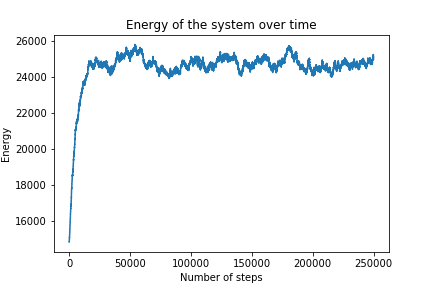
\includegraphics[width=0.7\textwidth]{../images/q1a_energy.png}
	\caption{Plot of the energy of the system over 250000 steps of the process of randomly increasing the states of random particles depending on the energy and temperature of the system.}
	\label{fig:q1a_energy}
\end{figure}

\begin{figure}[H]
	\centering
	\begin{minipage}{0.49\linewidth}
		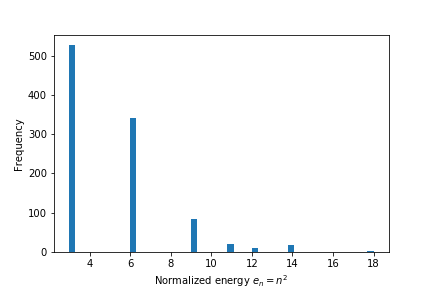
\includegraphics[width=\linewidth]{../images/q1a_energy_hist.png}
	\end{minipage}
		\begin{minipage}{0.49\linewidth}
		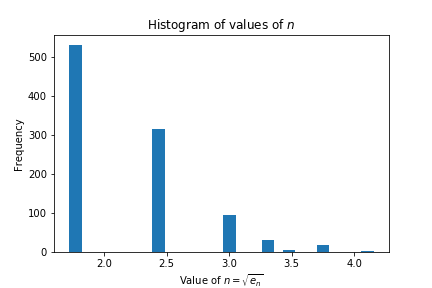
\includegraphics[width=\linewidth]{../images/q1a_n_hist.png}
	\end{minipage}
	\caption{Histograms of the distribution of values of the normalized energy $e_n = n^2$ (left) and the value of $n$ (right) for the system after 250,000 steps, when it is in equilibrium.}
	\label{fig:q1a_hist}
\end{figure}

\subsection{Part b)}

We seek to calculate the value of the total energy at equilibrium, and the average value of the quantum number $n$, for the system at various temperatures.

In order to achieve this, we adapted the code from part a) to iterate over the different temperatures desired, and run the Monte Carlo energy calculating scheme for each. In order to determine how long to run the simulation for at each temperature, we used a condition which would, at every 200,000th step, calculate the average energy across the most recent 200,000 steps and compare it to that of the previous set of 200,000 steps. Once the average energy of the more recent set of 200,000 steps is less than or equal to that of the previous set, we conclude that the system must have reached equilibrium, and stop iterating. The value of 200,000 was chosen from a combination of visual inspection of the size of the fluctuations in the energy and a component of trial and error.

\begin{figure}[H]
	\centering
	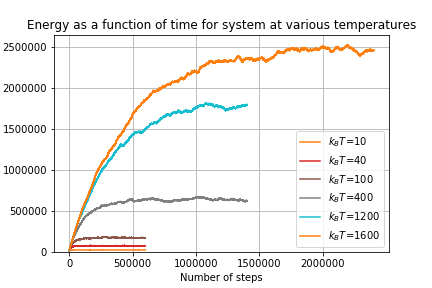
\includegraphics[width=0.8\textwidth]{../images/q1b_energies.png}
	\caption{Energy as a function of time for six different temperatures of the system, plotted until they reach equilibrium.}
	\label{fig:q1b_energies}
\end{figure}

\begin{figure}[H]
	\centering
	\begin{minipage}{0.49\linewidth}
		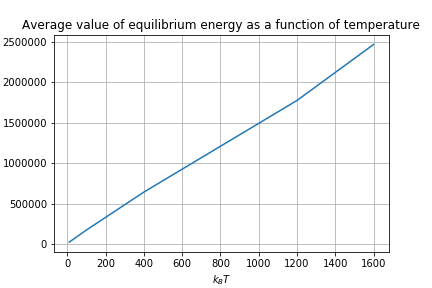
\includegraphics[width=\linewidth]{../images/q1b_av_energy.png}
		\caption{Equilibrium energy as a function of system temperature for the range of temperatures tested.}
		\label{fig:q1b_av_energy}
	\end{minipage}
	\begin{minipage}{0.49\linewidth}
		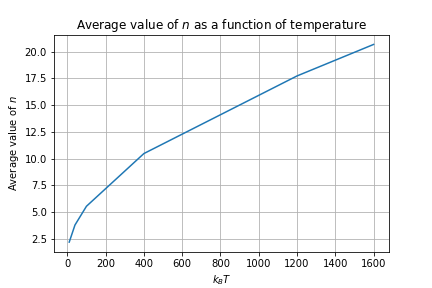
\includegraphics[width=\linewidth]{../images/q1b_av_n.png}
		\caption{Average value of $n$ as a function of system temperature for the range of temperatures tested.}
		\label{fig:q1b_av_n}
	\end{minipage}
\end{figure}

For each temperature, we computed the average value of $n$ using equation 5 from the handout, as well as stored the average value of the energy once the system reached equilibrium; these are plotted in figures \ref{fig:q1b_av_n} and \ref{fig:q1b_av_energy}, respectively. From the slope of the graph in figure \ref{fig:q1b_av_energy}, we calculate that the value of $\Delta E / \Delta T$ over the range of temperatures tested is approximately:
\begin{equation}
	\frac{\Delta E}{\Delta T} \approx 1535
\end{equation}

\section{Ising Model}

We seek to create a program which runs a Metropolis-style Monte Carlo simulation of the Ising model
of a magnet and calculates the total magnetization of the system over time. The
program also plots the state of the system at a subset of the timesteps to
create an animation of the magnetization process.

The program written to do this is included in the file Lab11\_Q2.py. Initially, the array of dipoles is created with random orientations of either $+1$ or $-1$ at each point. The program then iterates over the specified number of steps, at each step randomly choosing one dipole to flip, computing the new energy with the flipped dipole, and then deciding whether to keep or reject the flip based on the Metropolis acceptance formula (10.60 from Newman). The total magnetization of the system, which is just the sum of all the dipole orientations, is then plotted as a function of time. The program was run several times with $T=1$; in each instance, the total magnetization would start near zero, since the sum of the 400 random initial values should be about zero, and then drifts randomly before eventually moving to one extreme value or the other, either $+400$ or $-400$, which correspond to all of the spins being either up or down, respectively (examples shown in figure \ref{fig:q2_magnetization}). This makes sense, as the system prefers to move into states with lower energy (as given by equation \ref{eq:energy}), and the energy of a given pair of dipoles is higher when they are anti-aligned and lower when they are aligned. Hence, the system starts near zero total magnetization, at which point the total change is effectively random, but once it drifts far enough to one side such as to make the chances of aligning with the dominant existing alignment sufficiently favourable, that alignment ``takes over'' the whole system and it settles into its ground state.

\begin{equation}
	E = -J\sum_{\langle ij \rangle}s_i s_j
	\label{eq:energy}
\end{equation}

\begin{figure}[H]
	\begin{minipage}{0.49\linewidth}
		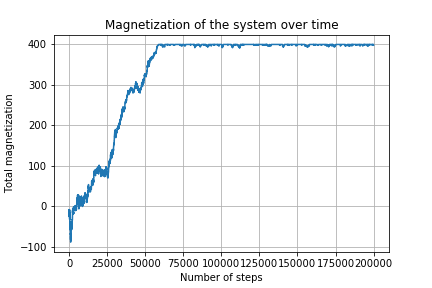
\includegraphics[width=\linewidth]{../images/q2_magnetization_pos.png}
	\end{minipage}
	\begin{minipage}{0.49\linewidth}
		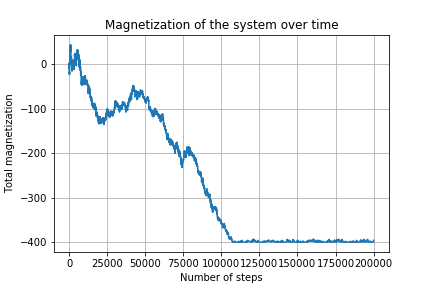
\includegraphics[width=\linewidth]{../images/q2_magnetization_neg.png}
	\end{minipage}
	\caption{Plots of total magnetization of the system over time. The system can spontaneously drift to either a completely positive (left) or completely negative (right) magnetization, with an equal chance of either occurring, based on the initial conditions and early random dipole flips.}
	\label{fig:q2_magnetization}
\end{figure}

Running the simulation for one million time steps for three different temperatures, $T=(1,2,3)$, we produced the graphs of total magnetization over time presented in figures \ref{fig:q2_mag_T=1}, \ref{fig:q2_mag_T=2}, and \ref{fig:q2_mag_T=3}. For each temperature, an animation of the state of the system over time was produced using matplotlib.animation. In the case of $T=1$, we could observe that the system would start with all of the dipoles at random values, looking somewhat like a checker board, and would quickly coalesce into groups of adjacent dipoles all having the same orientation in close proximity to each other, producing a pattern like the spots on a cow. Then these groups would slowly grow larger or smaller, and as soon as one orientation became significantly more prevalent than the other, the dominant one would ``take over'' the whole system. Dipoles in the middle of established groups would occasionally flip their signs, but these changes would be quickly reversed.

In the case of $T=2$, the same general behaviour was repeated, although there was far more noise present in the system, with random dipoles flipping and staying flipped much more often. This makes sense, given that at higher temperature the probability of accepting a move which increases the energy of a system is higher, as described by the Metropolis acceptance formula that we used. Indeed, as we can see from figure \ref{fig:q2_mag_T=2}, the system did establish a general preference for one orientation in particular, (negative/down in the case shown), but there was still a large number of dipoles pointing the opposite direction at any given time, which would continue to pop up and then flip back as others did the same.

For $T=3$, as we can see from figure \ref{fig:q2_mag_T=3}, the probability of accepting moves that increase energy seems to be high enough such as to prevent the system from ever settling into any equilibrium. Indeed, this was borne out by the animation as well, where the system effectively just looked like television static, with random dipoles flipping back and forth with no structure at all, and with the average total magnetization staying around zero.

\begin{figure}[H]
	\centering
	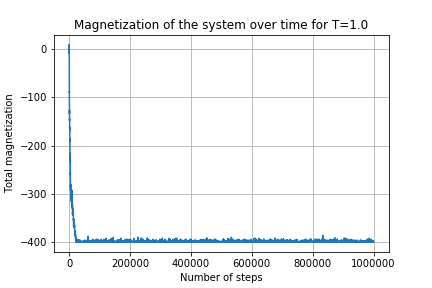
\includegraphics[width=0.8\textwidth]{../images/q2_magnetization_T=1.png}
	\caption{Plot of total system energy as a function of time for the system when $T=1$.}
	\label{fig:q2_mag_T=1}
\end{figure}

\begin{figure}[H]
	\centering
	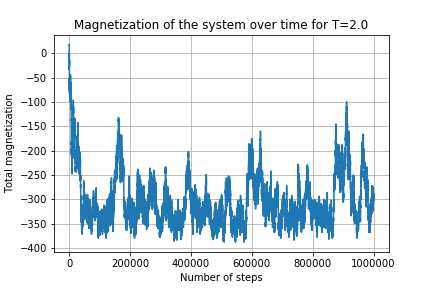
\includegraphics[width=0.8\textwidth]{../images/q2_magnetization_T=2.png}
	\caption{Plot of total system energy as a function of time for the system when $T=2$.}
	\label{fig:q2_mag_T=2}
\end{figure}

\begin{figure}[H]
	\centering
	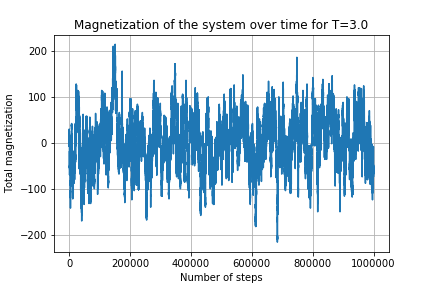
\includegraphics[width=0.8\textwidth]{../images/q2_magnetization_T=3.png}
	\caption{Plot of total system energy as a function of time for the system when $T=3$.}
	\label{fig:q2_mag_T=3}
\end{figure}

\section{Simulated Annealing Warm-up}
For this question the desire is to observe the behaviors of a simulated annealing problem. A provided program uses simulated annealing by choosing a set of points and then calculating the shortest round trip, going through each point only once. We modified the program in such a way as to fixed the set of points over the course of several runs using a fixed seed of $1$ for our pseudo-random number generator(PRNG), and then proceeded to alter the starting point of the optimization code using a unique random number seed for each run. Three of the resulting paths using seed of $50$, $100$, and $1000$ are shown in figure \ref{fig:q3_seeds}. Running the program with 10 different seeds resulted in a distance measure that ranged from ca. $D=4.77$ to $D=5.53$ as a result from taking different final paths. 
We then chose a fixed optimization path using the seed of $100$ and decreased the scheduling time scale $\tau$ from $1e4$ in figure \ref{fig:q3_seeds} to $1e3$ in figure \ref{fig:q3_t=1000}. Comparing the two results, the one with a short scheduling time $\tau=1e3$ took less time to solve however we can see from the images that the resulting path is not as optimized. The shorter scheduling time resulted in a much larger final distance of ca. $D=5.78$ which exceeds our seed dependent range previously stated. Using the same path seed again, we then increased the time scale to $\tau=2e4$ and the resulting path and distance is shown in figure \ref{fig:q3_t=20000}. We initially increased the time scale to $tau=1e5$ however this resulted in a run time that seems indefinite. Even just doubling the time scale resulted in a much higher run time and from figures \ref{fig:q3_seeds} and \ref{fig:q3_t=20000} we can see the final path of the larger scheduling time scale actually results in a longer distance of $D=5.16$. Thus for our data is seems that increasing or decreasing the cooling time results in worse optimized solution with a larger distance than that using a cooling time of $\tau=1e4$. 

\begin{figure}[H]
	\begin{minipage}{0.49\linewidth}
		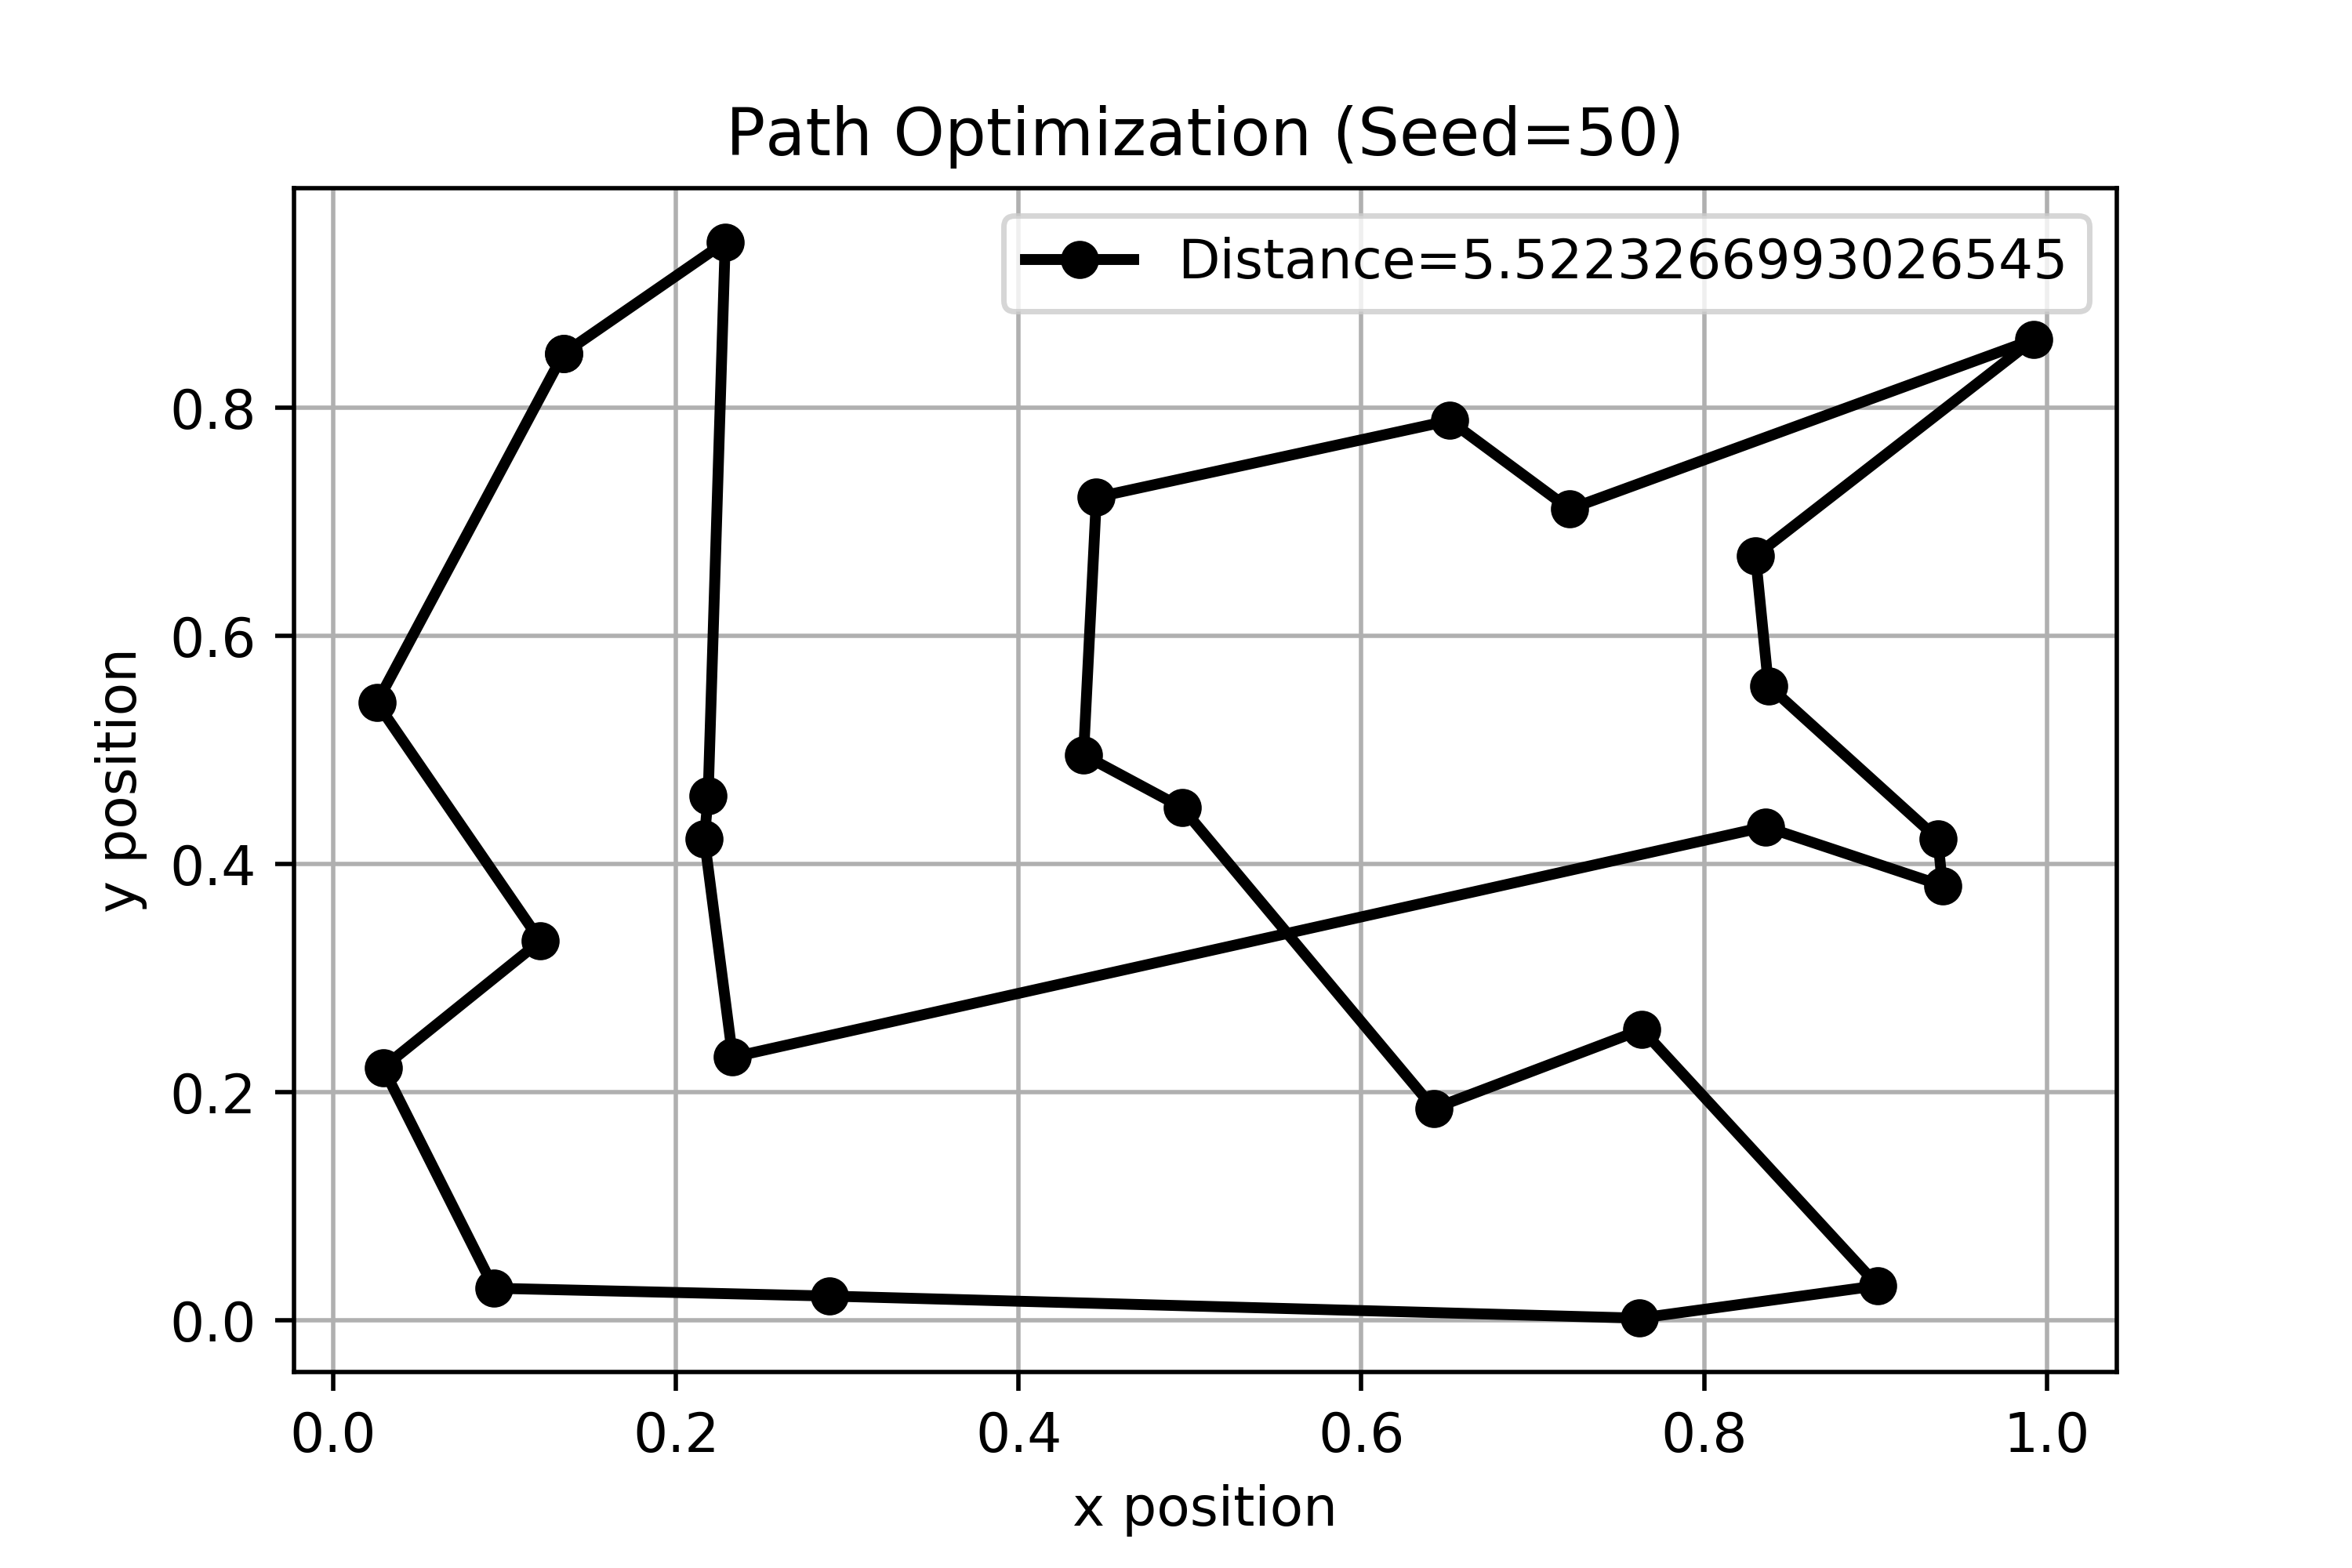
\includegraphics[width=\linewidth]{../images/q3_s=50.png}
	\end{minipage}
	\begin{minipage}{0.49\linewidth}
		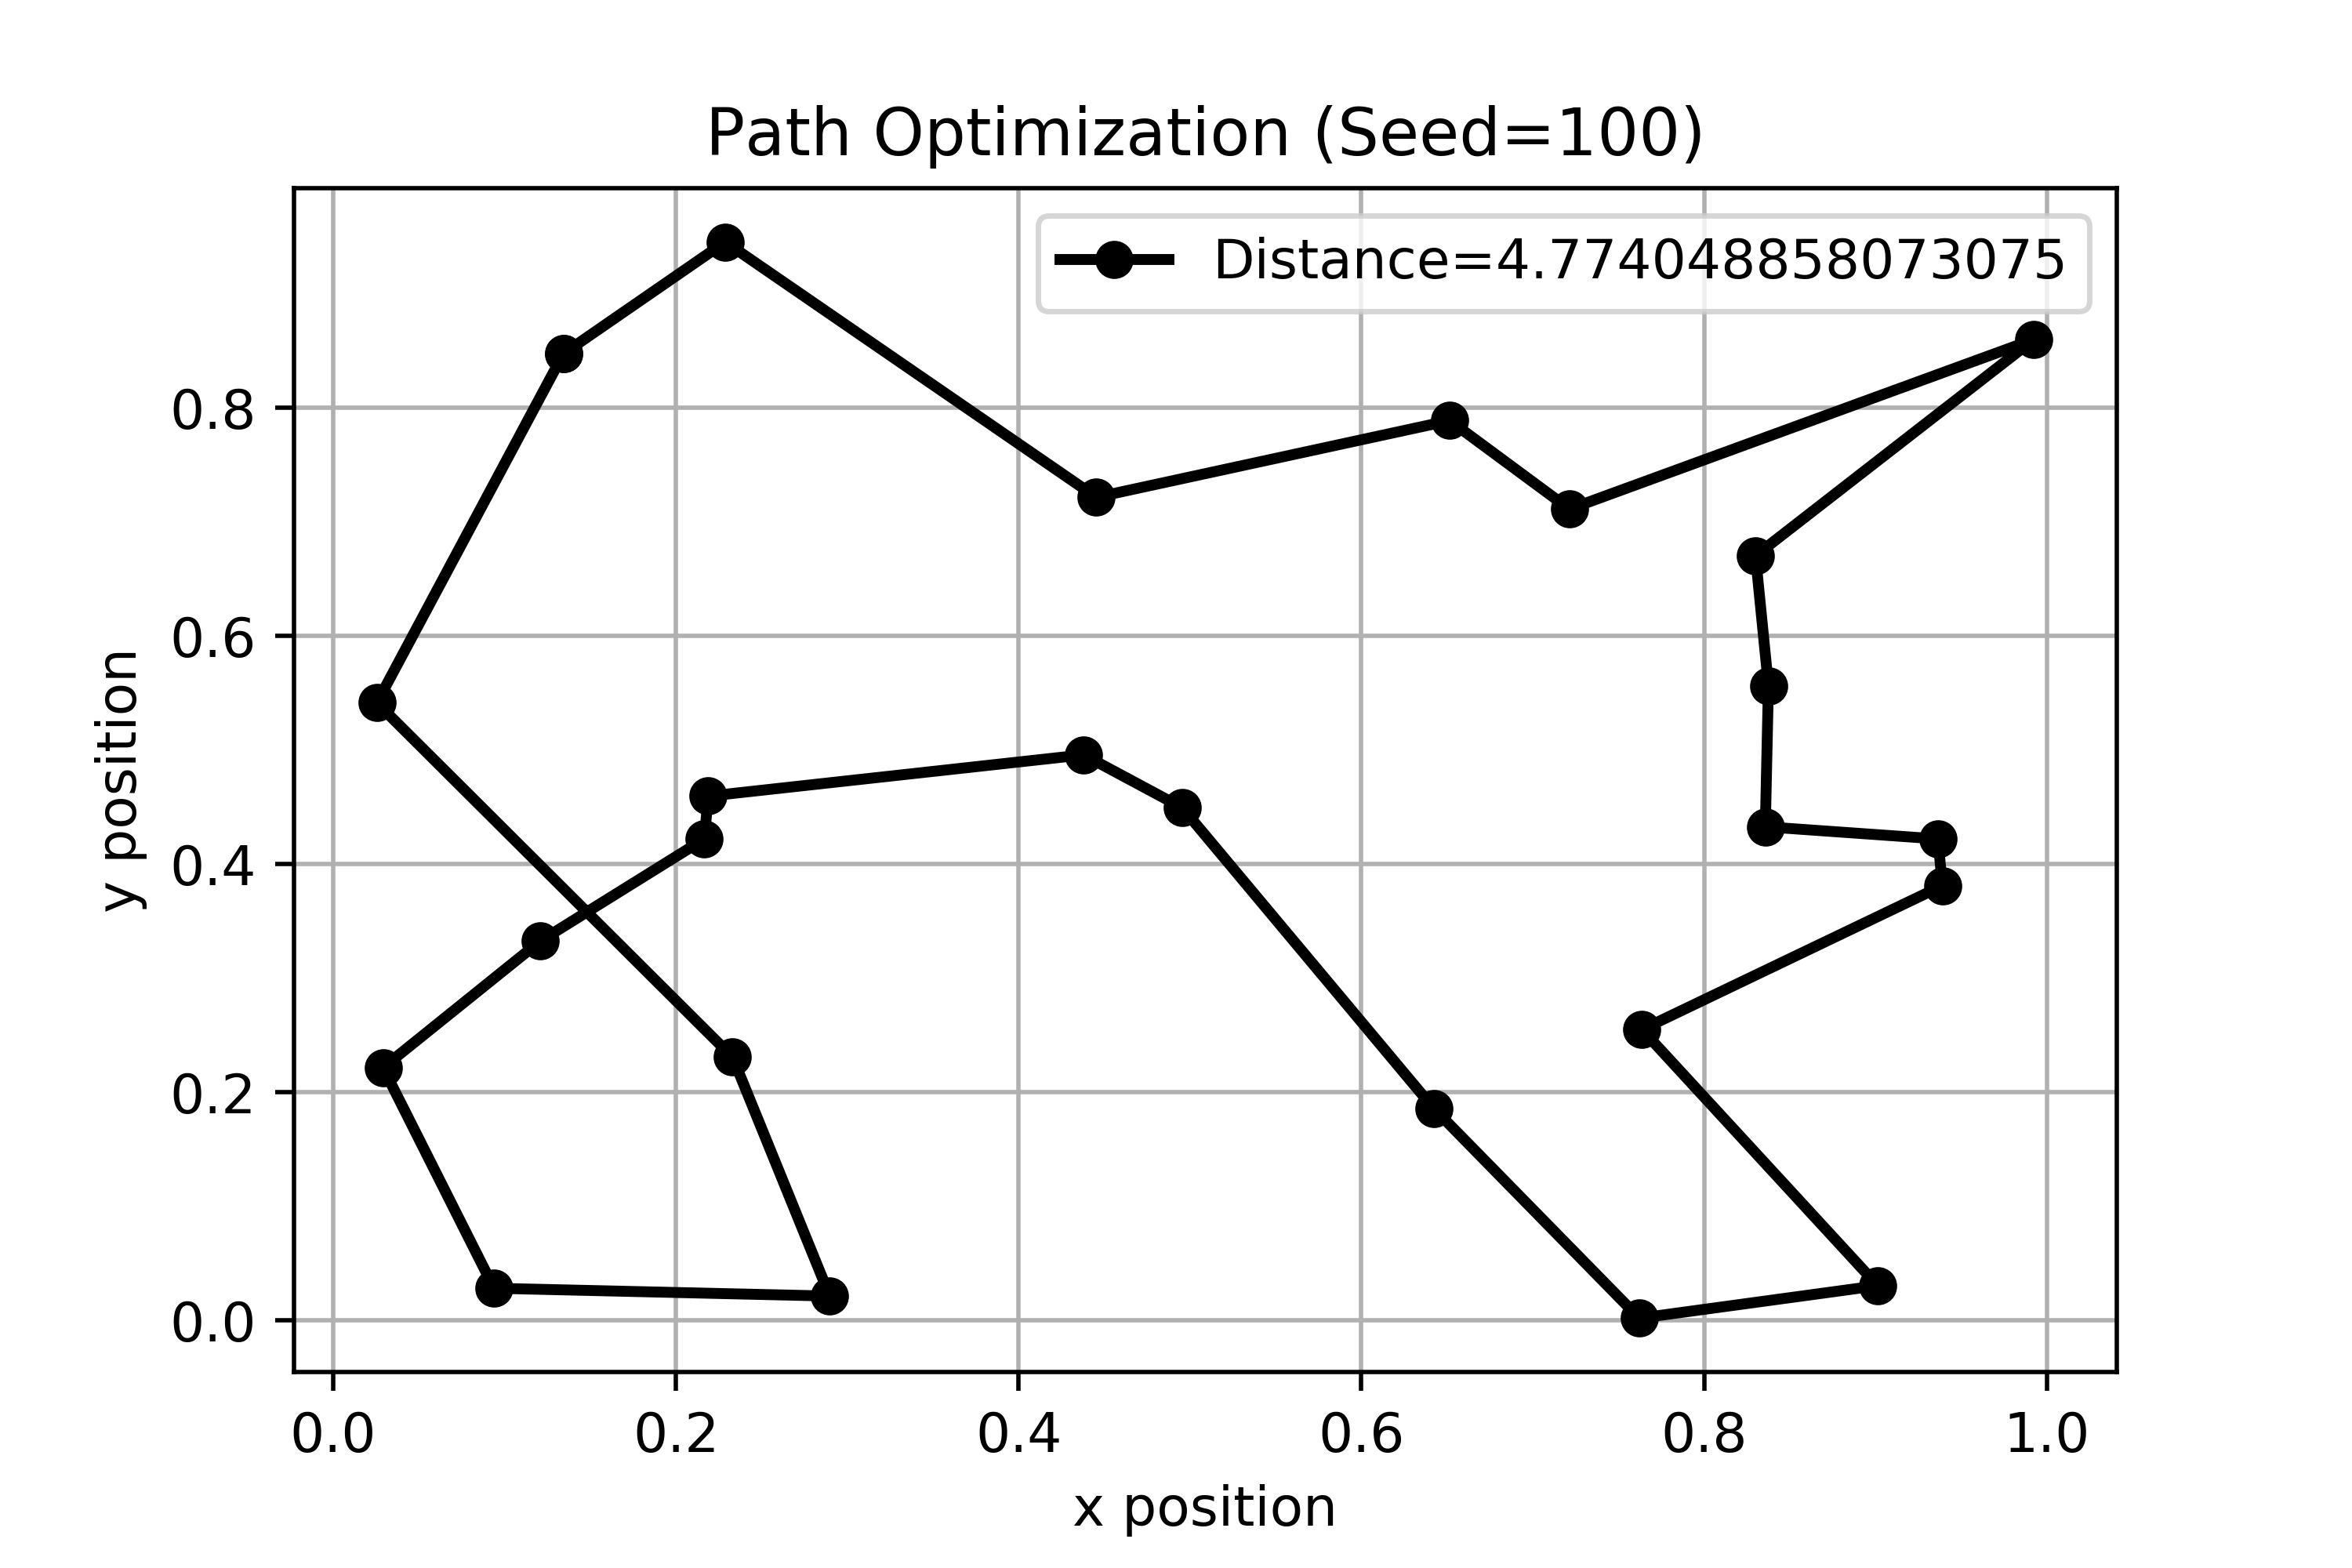
\includegraphics[width=\linewidth]{../images/q3_s=100.png}
	\end{minipage}
	\centering
	\begin{minipage}{0.49\linewidth}
		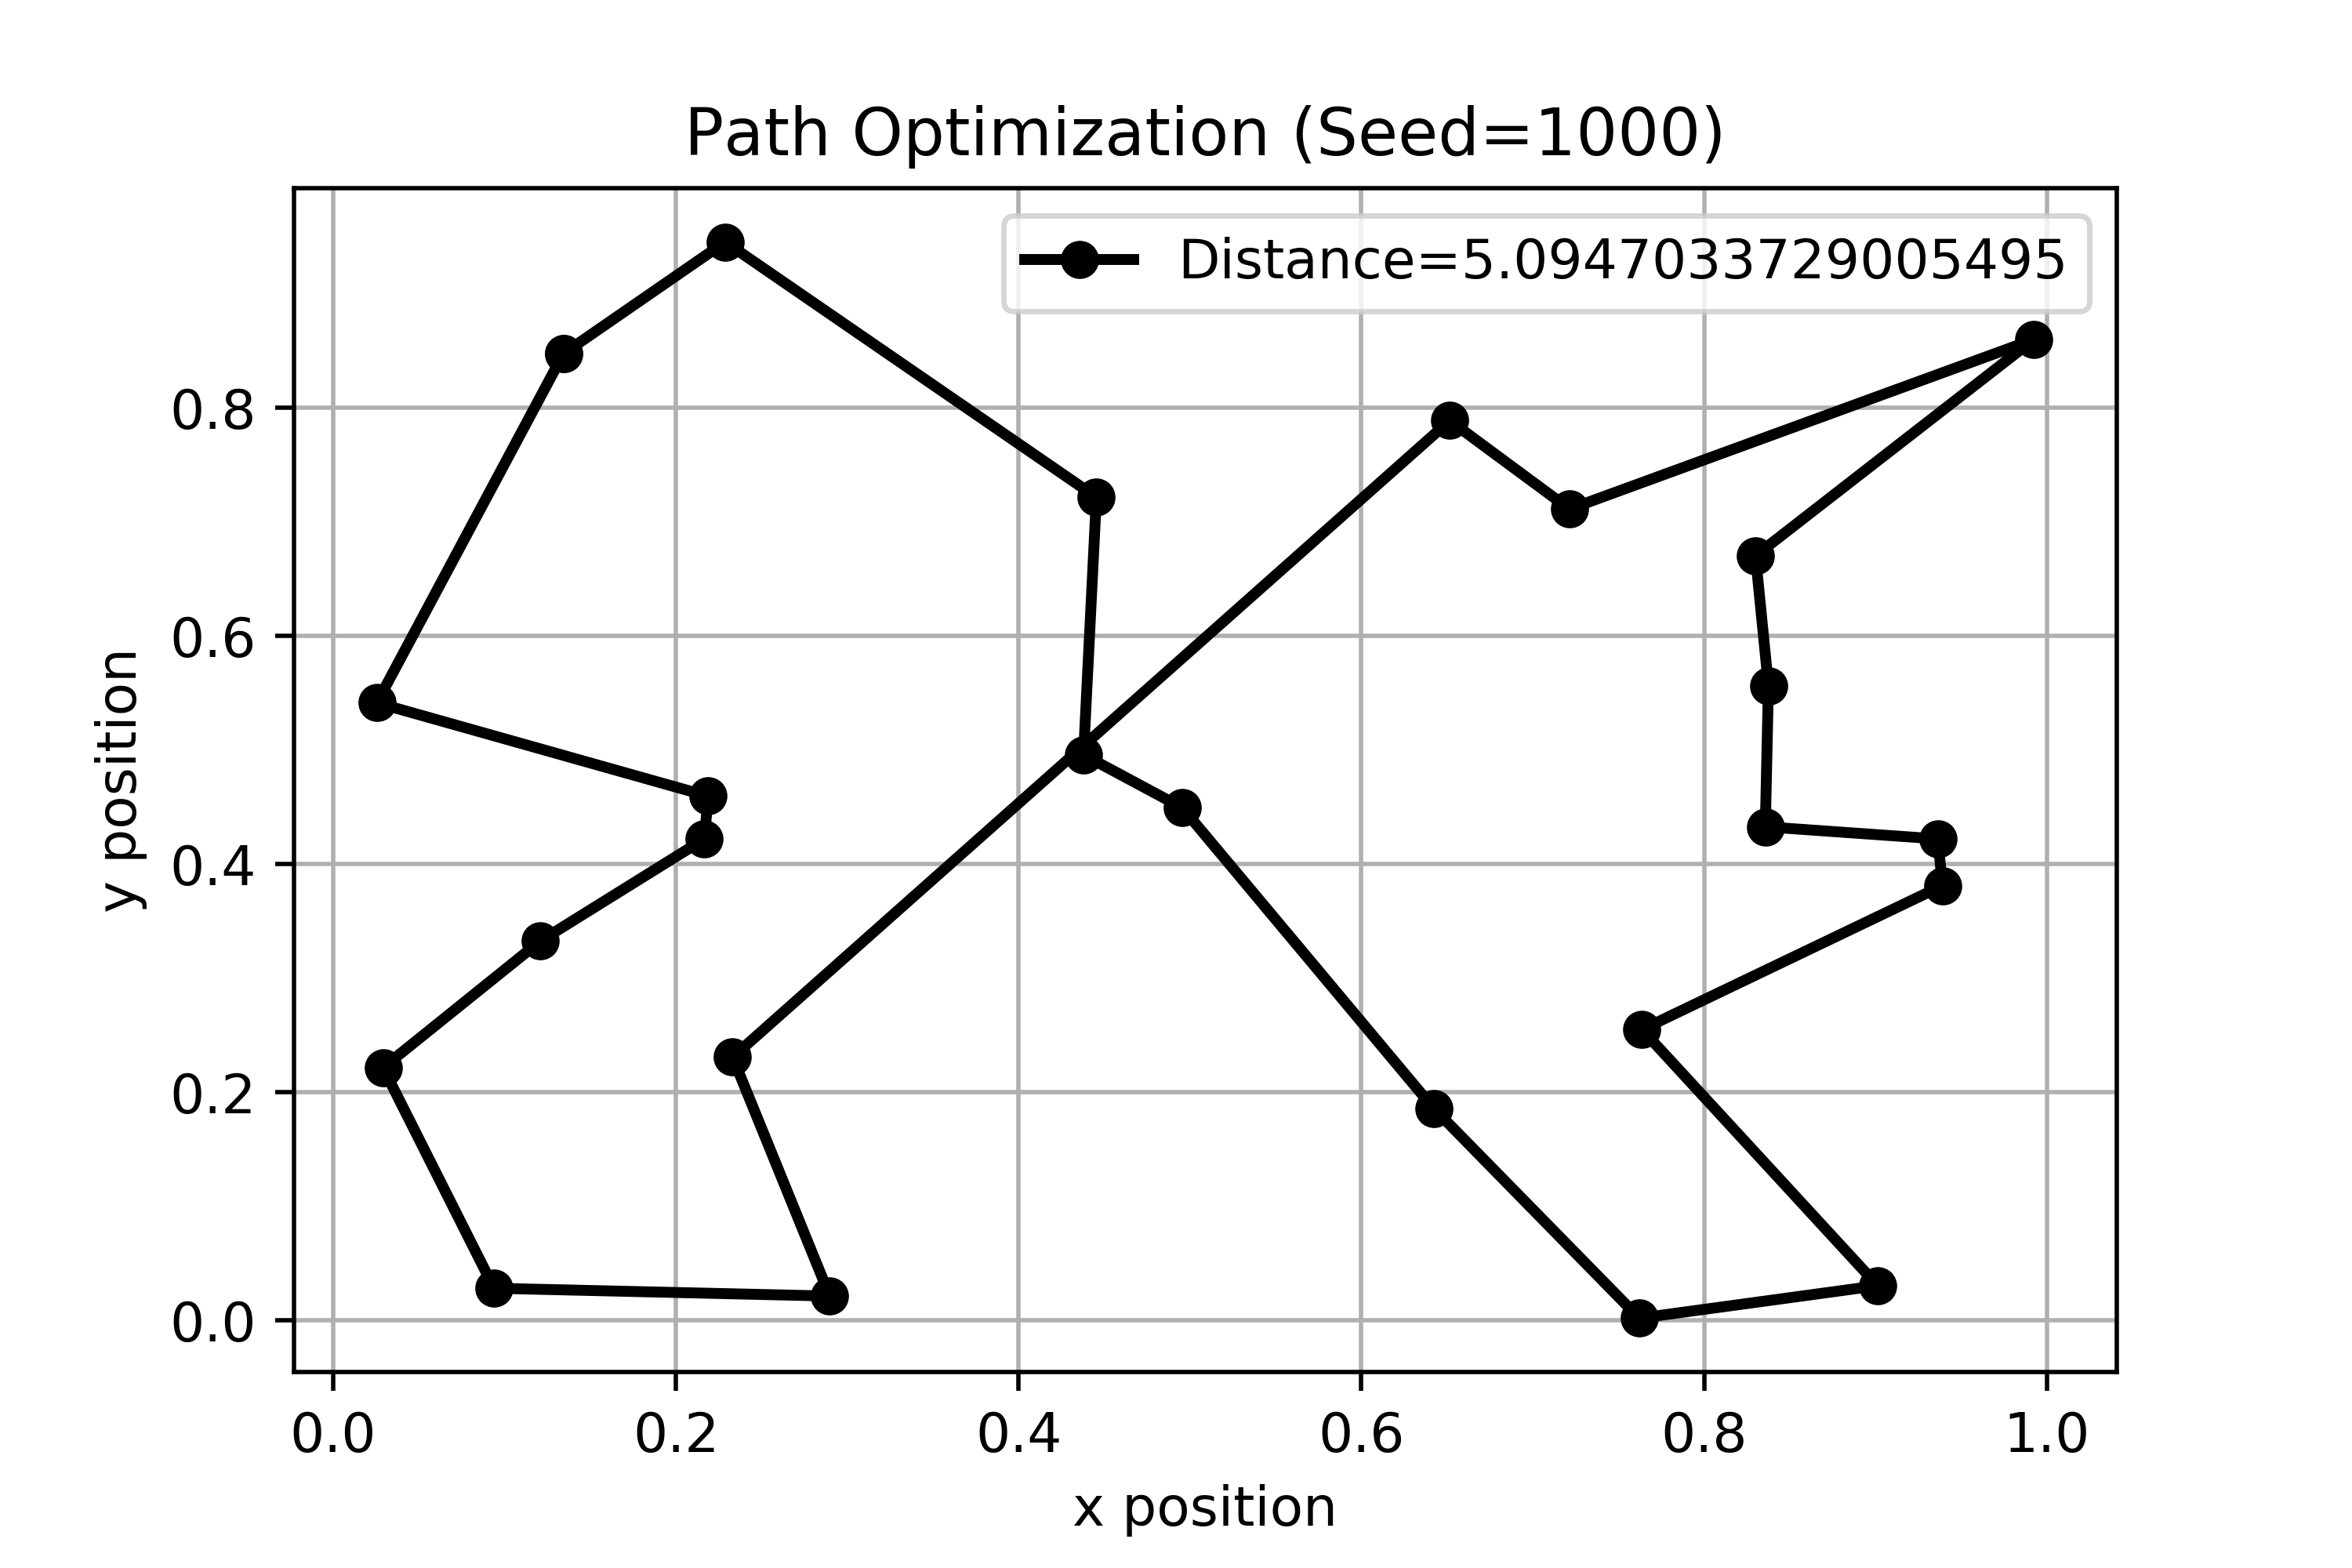
\includegraphics[width=\linewidth]{../images/q3_s=1000.png}
	\end{minipage}
	\caption{Plots showing various optimizations to the Traveling salesman problem.}
	\label{fig:q3_seeds}
\end{figure}

\begin{figure}[H]
	\centering
	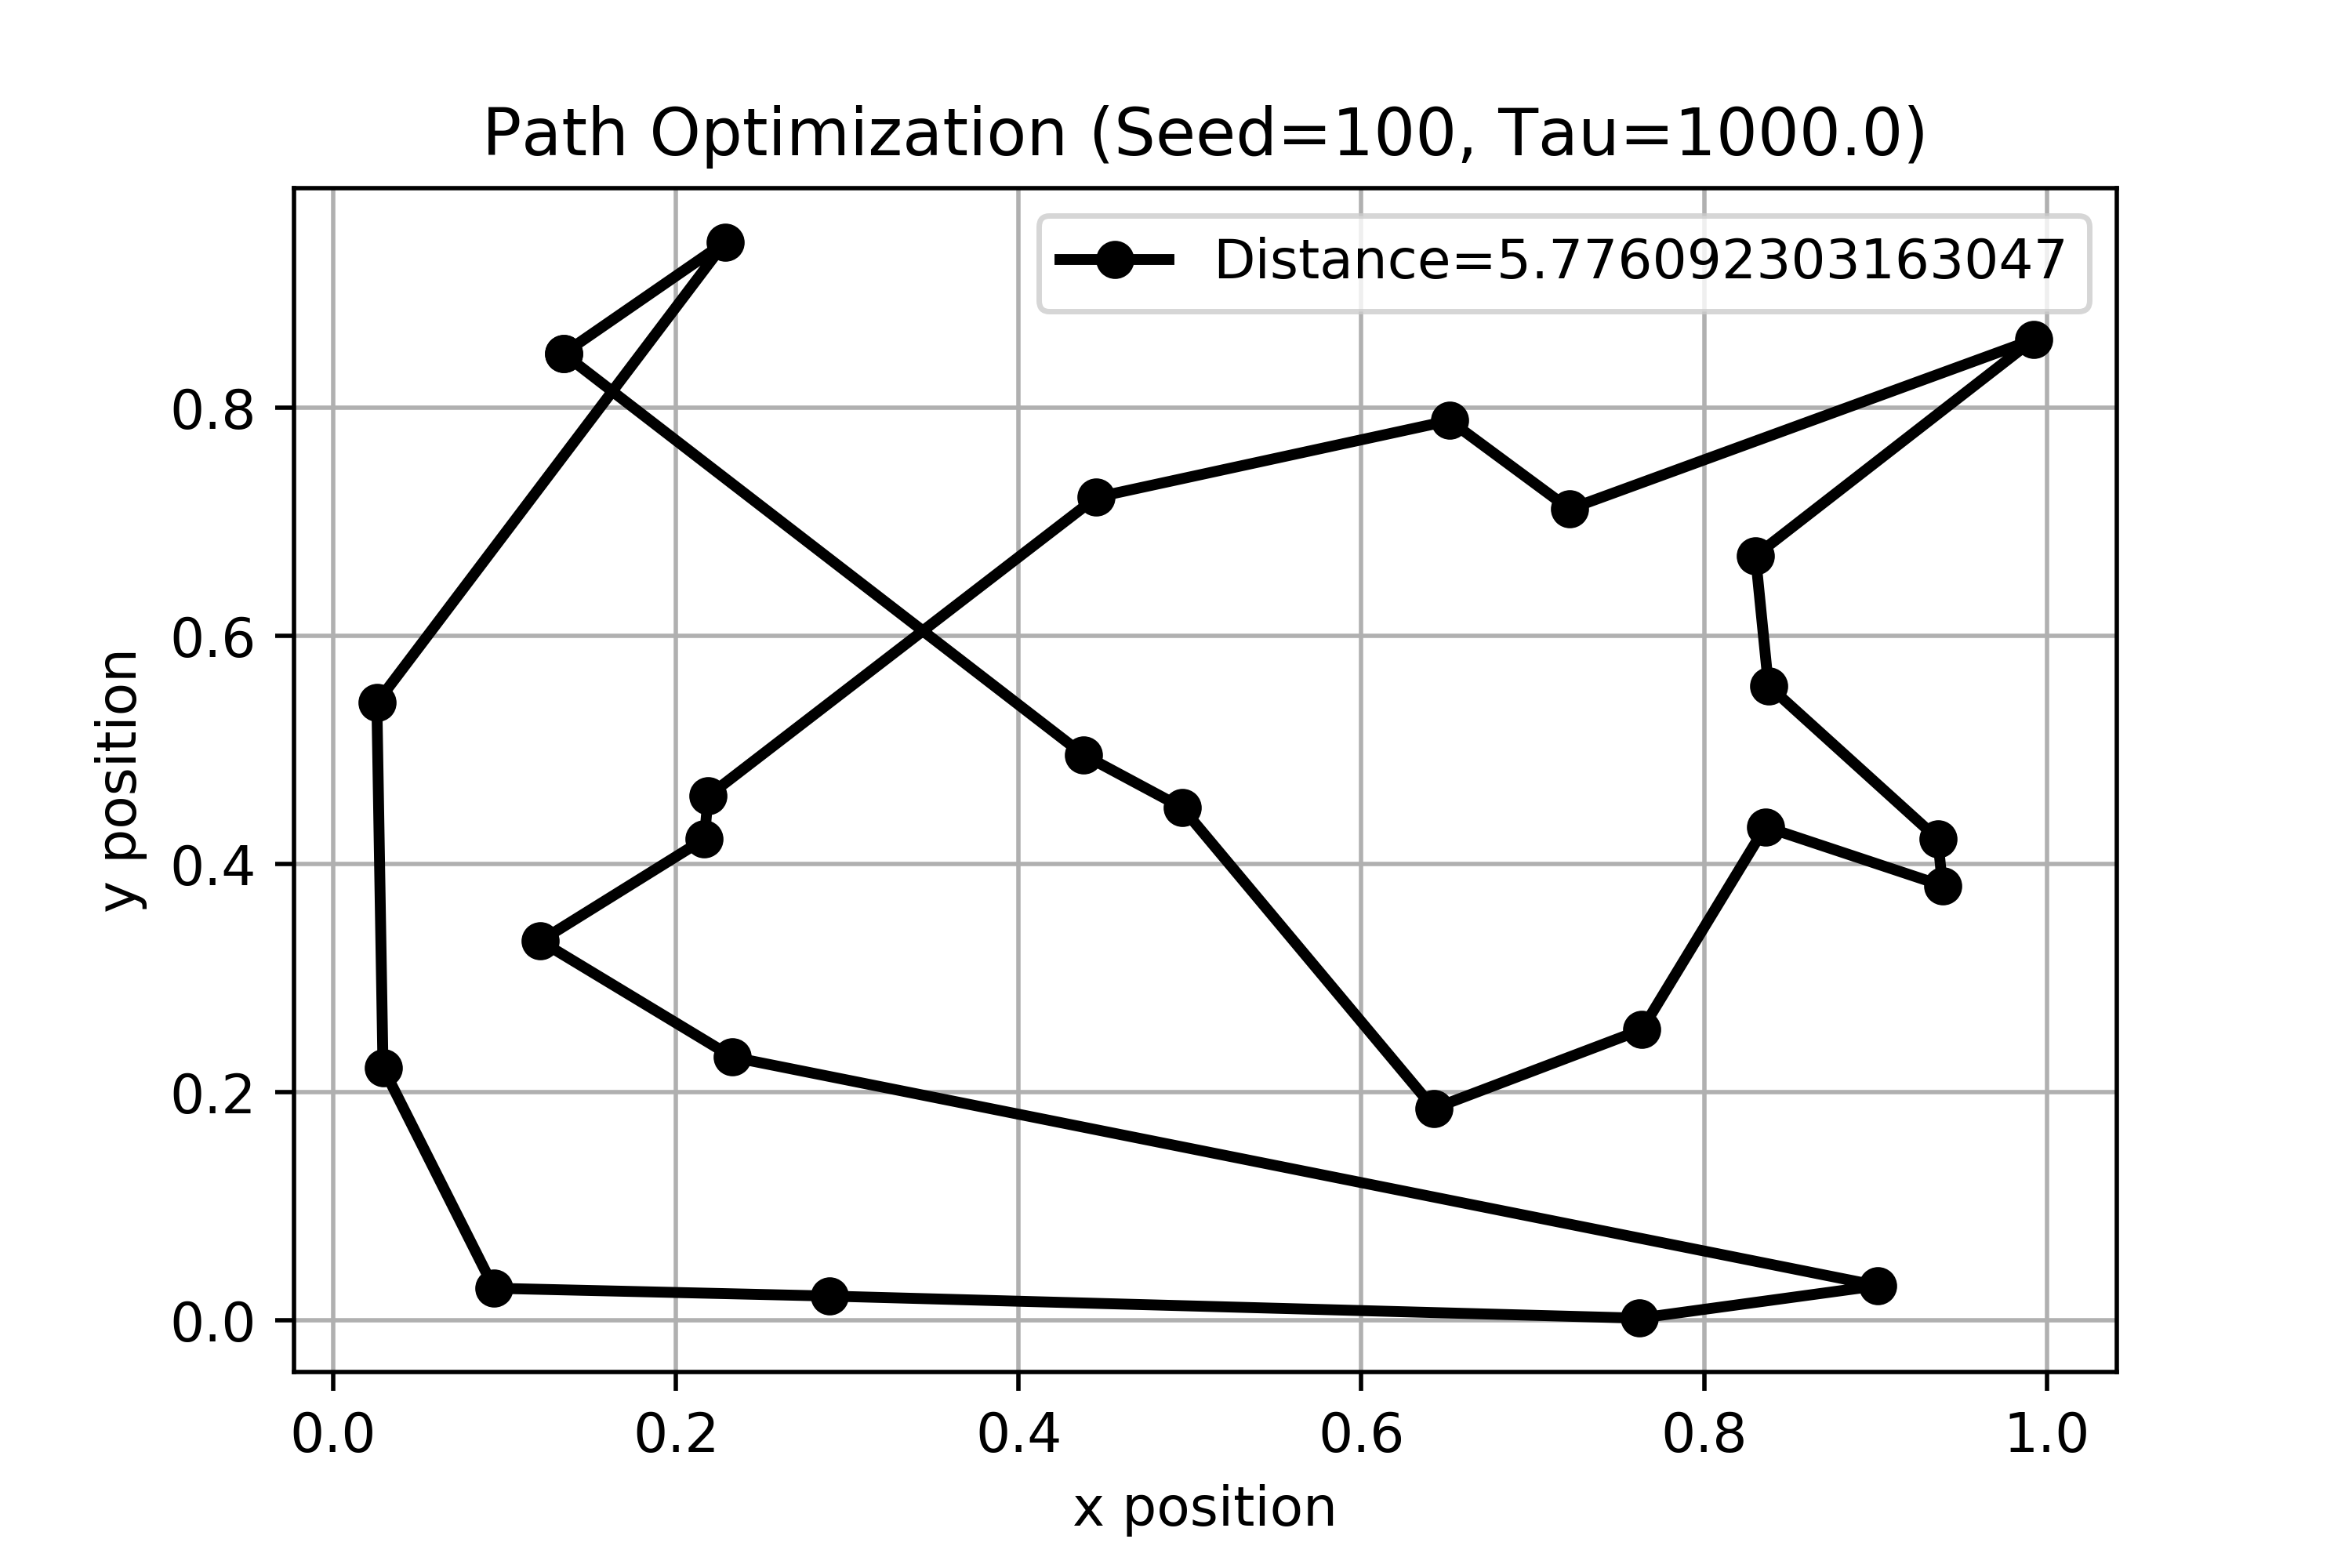
\includegraphics[width=\linewidth]{../images/q3_s=100_t=1000.png}
	\caption{Plots showing the same optimization path as the second image of figure \ref{fig:q3_seeds} but with a short scheduling time parameter.}
	\label{fig:q3_t=1000}
\end{figure}

\begin{figure}[H]
	\centering
	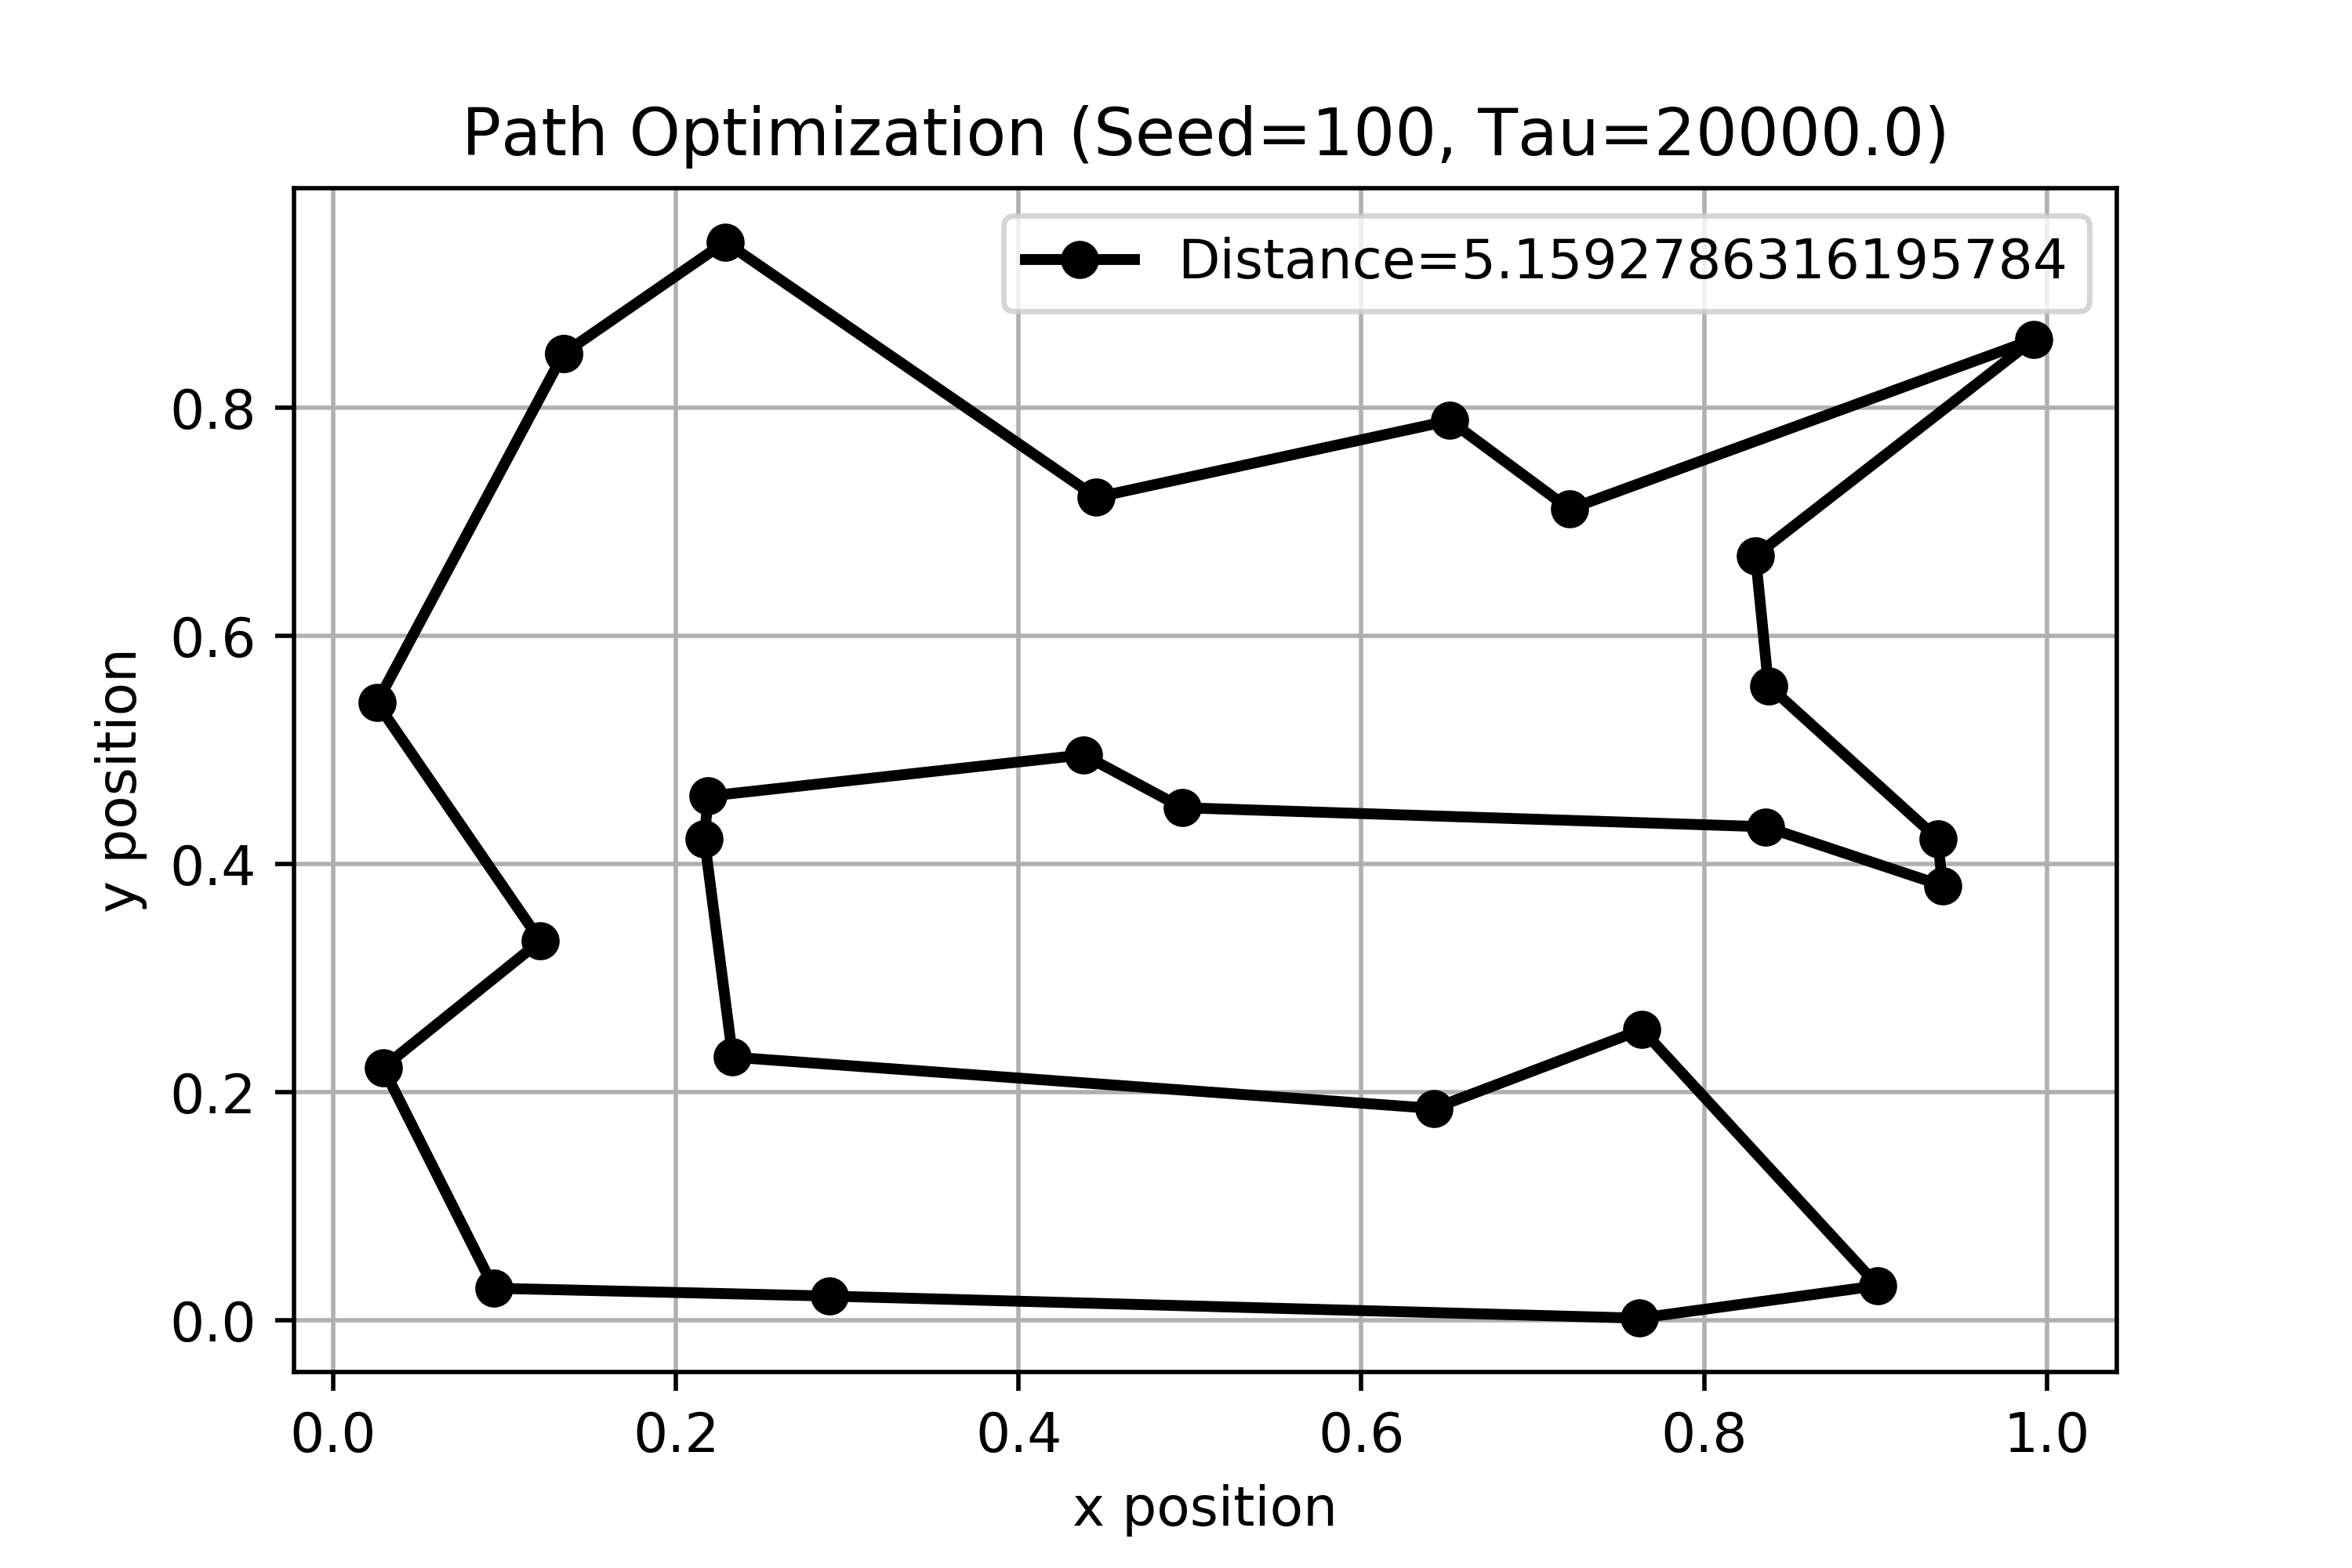
\includegraphics[width=\linewidth]{../images/q3_s=100_t=20000.png}
	\caption{Plots showing the same optimization path as the second image of figure \ref{fig:q3_seeds} but with a longer scheduling time parameter.}
	\label{fig:q3_t=20000}
\end{figure}

\section{Dimer Covering Problem}
For this question we seek to solve a problem analogous to the dimer covering problem found in condensed matter physics. We do this by simplifying our problem such that our surface is a square grid and the dimers are objects that take up 2 adjacent points on the grid. For our program we use a pseudo-random number generator (PRNG) to randomly choose where on the grid the dimers will be placed. Using a fixed seed we can simulate the problem in a repeatable manner such that we can later alter parameters of the data to get new results. Once the dimers have a randomly chosen set of coordinates, we check to see if the space is occupied. If the space is free then the dimer is placed there and if the new dimer coincides with a previous one than the placed dimer is removed depending on a given Boltzmann probability. The resulting covers for time scale values of $\tau = 10^4, 10^3, 10^2, 10$ are shown in figures \ref{fig:q4_dimers_t=1e4}, \ref{fig:q4_dimers_t=1e3}, \ref{fig:q4_dimers_t=1e2}, and \ref{fig:q4_dimers_t=1e1} respectively. We can see that as our time scale is decreased the total number of covering dimers is significantly decreased. We then plotted the energy of the systems as a function of time where each dimer placed on the grid contributes a energy of $-1$ and each newly spawned dimer (not necessarily placed) counts as a time step. The energy plots of the corresponding covers are shown in figures \ref{fig:q4_dimers_t=1e4}, \ref{fig:q4_dimers_t=1e3}, \ref{fig:q4_dimers_t=1e2}, and \ref{fig:q4_dimers_t=1e1}. From these plots we can see that for a small enough time scale the energy curve appears linear since it only contains a small sample of the large time scale energy curve. As the time scale is increased and the grid begins to fill up, the program tends towards removing and adding dimers at a similar rate resulting to a curve that exhibits reciprocal behavior. We note that for $\tau=10^4$ the energy curve starts to show noise below $E=-800$ presumably due to the behavior of the PRNG and the probability of removing dimers.

\begin{figure}[H]
	\begin{minipage}{0.49\linewidth}
		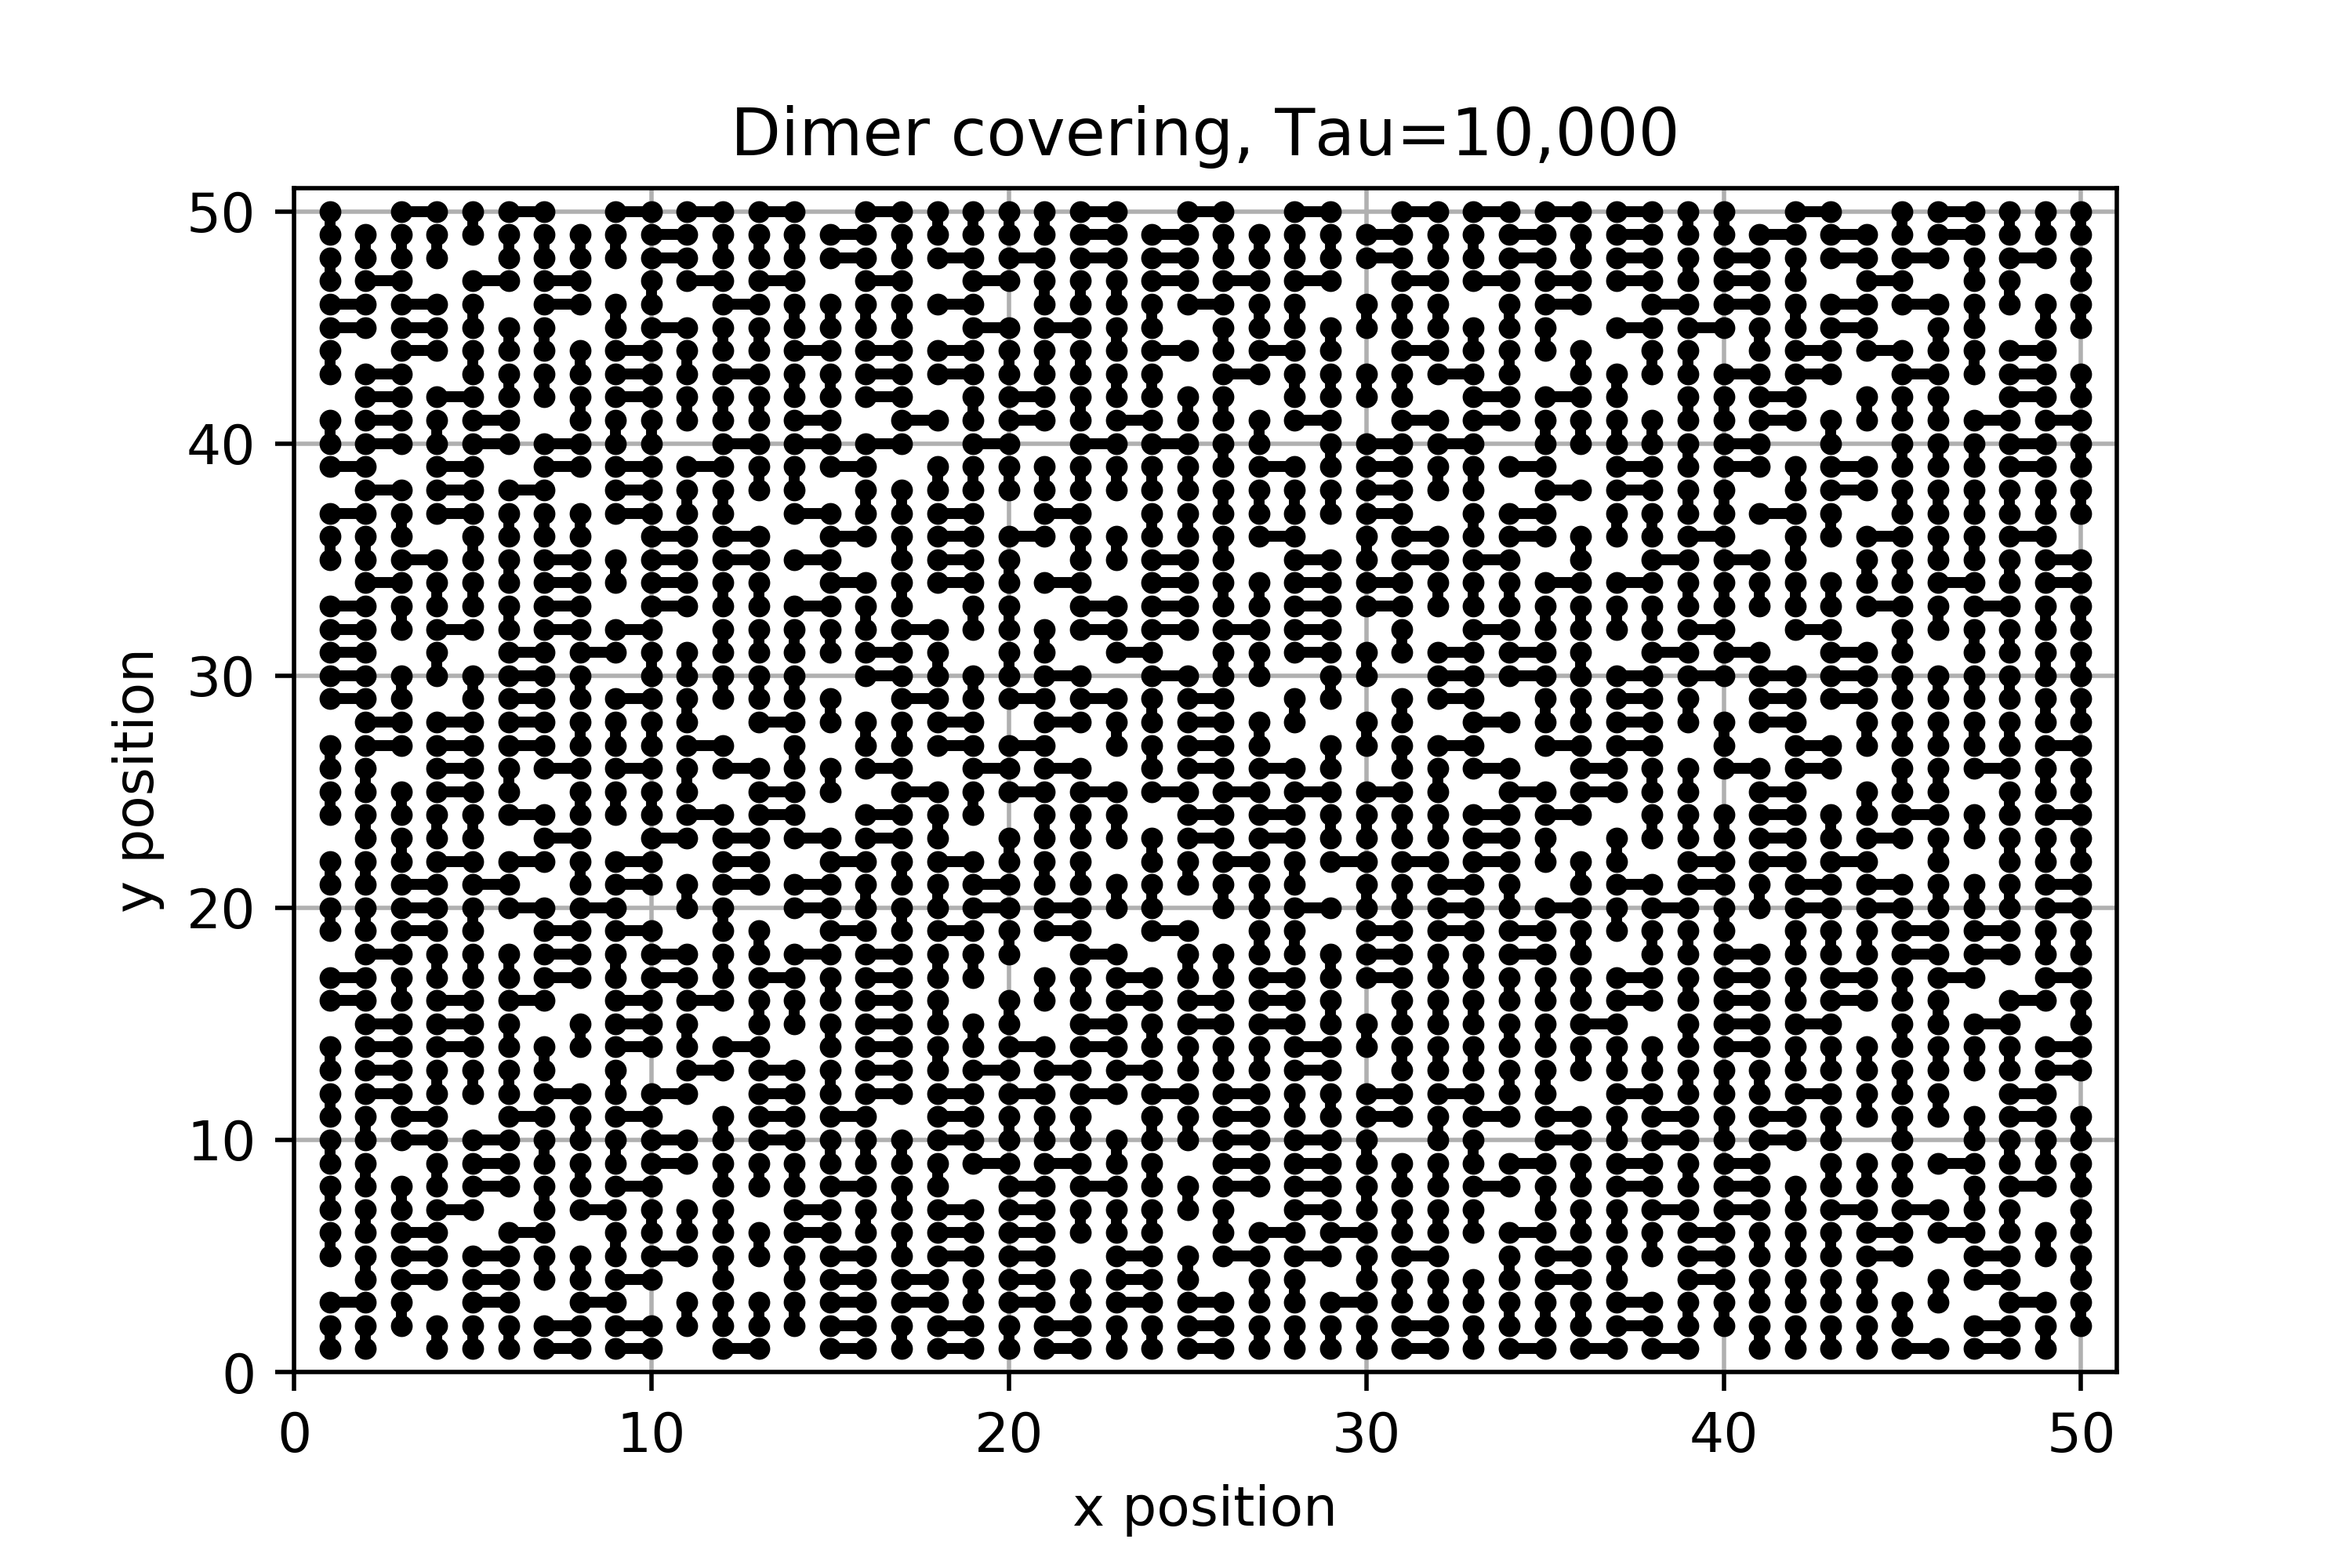
\includegraphics[width=\linewidth]{../images/q4_dimers_t=1e4.png}
	\end{minipage}
	\begin{minipage}{0.49\linewidth}
		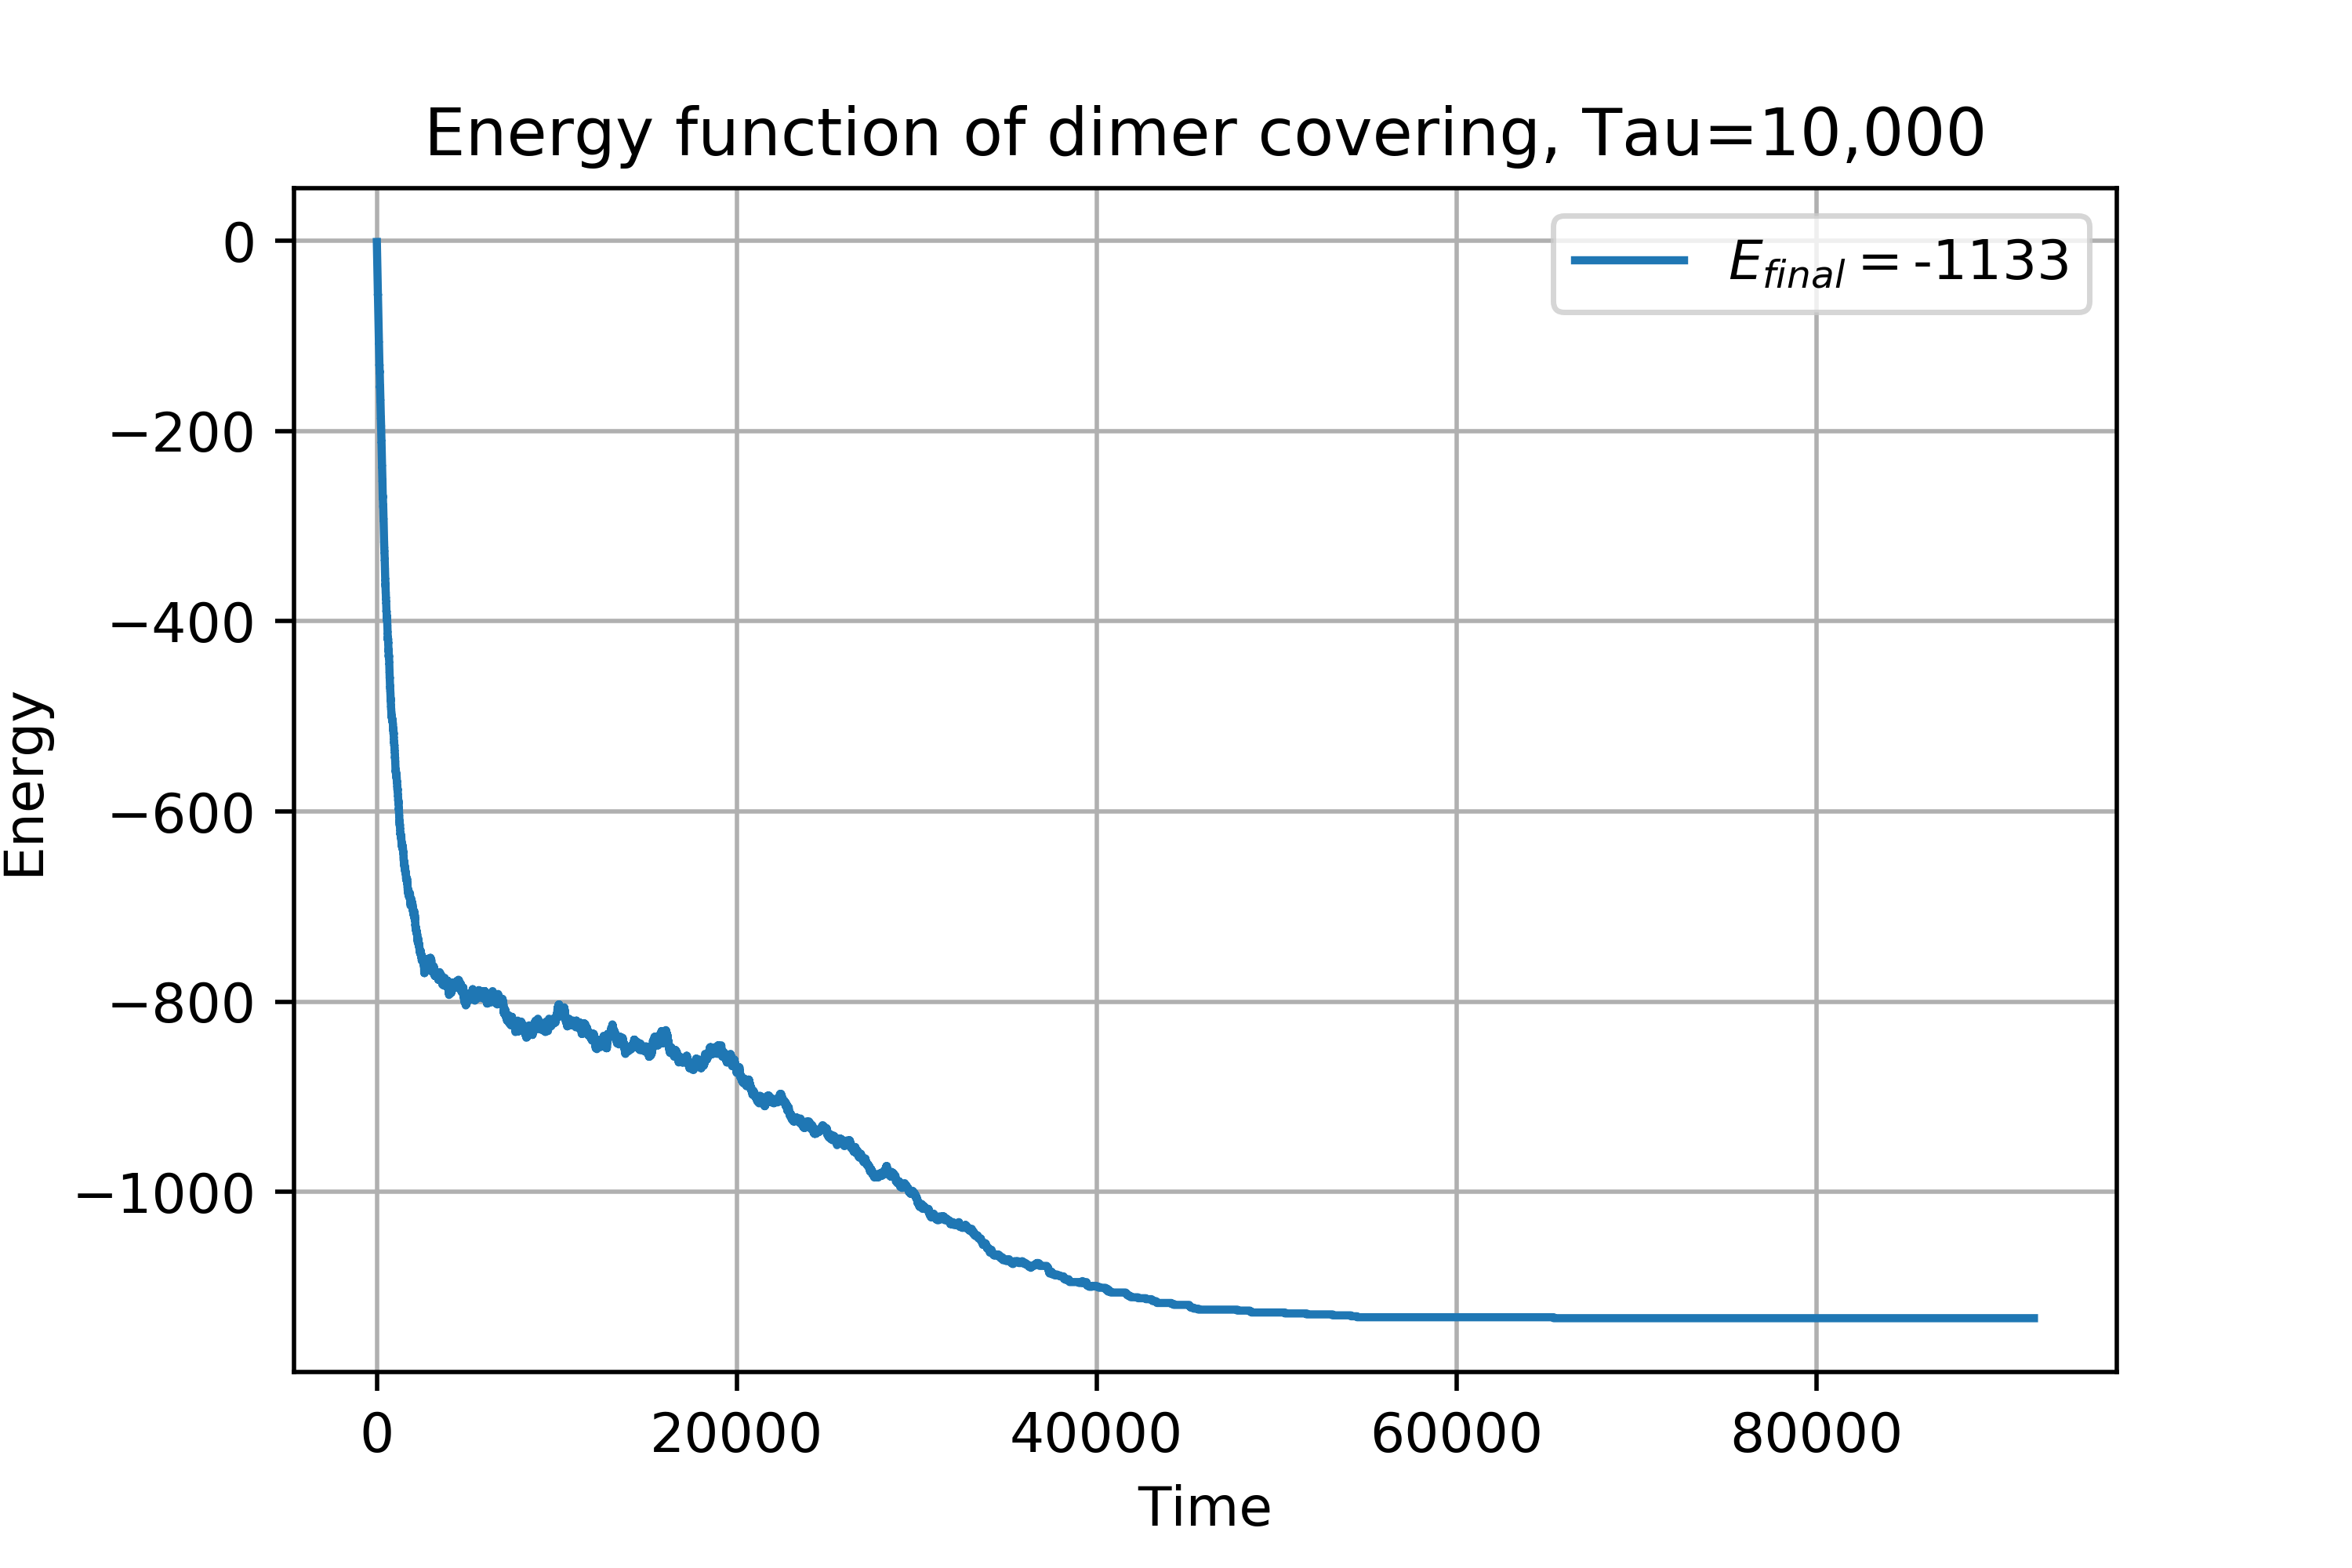
\includegraphics[width=\linewidth]{../images/q4_energy_t=1e4.png}
	\end{minipage}
	\caption{Dimer covering and corresponding energy curve as a result of simulated annealing with a time scale of $\tau = 10^4$}
	\label{fig:q4_dimers_t=1e4}
\end{figure}

\begin{figure}[H]
	\begin{minipage}{0.49\linewidth}
		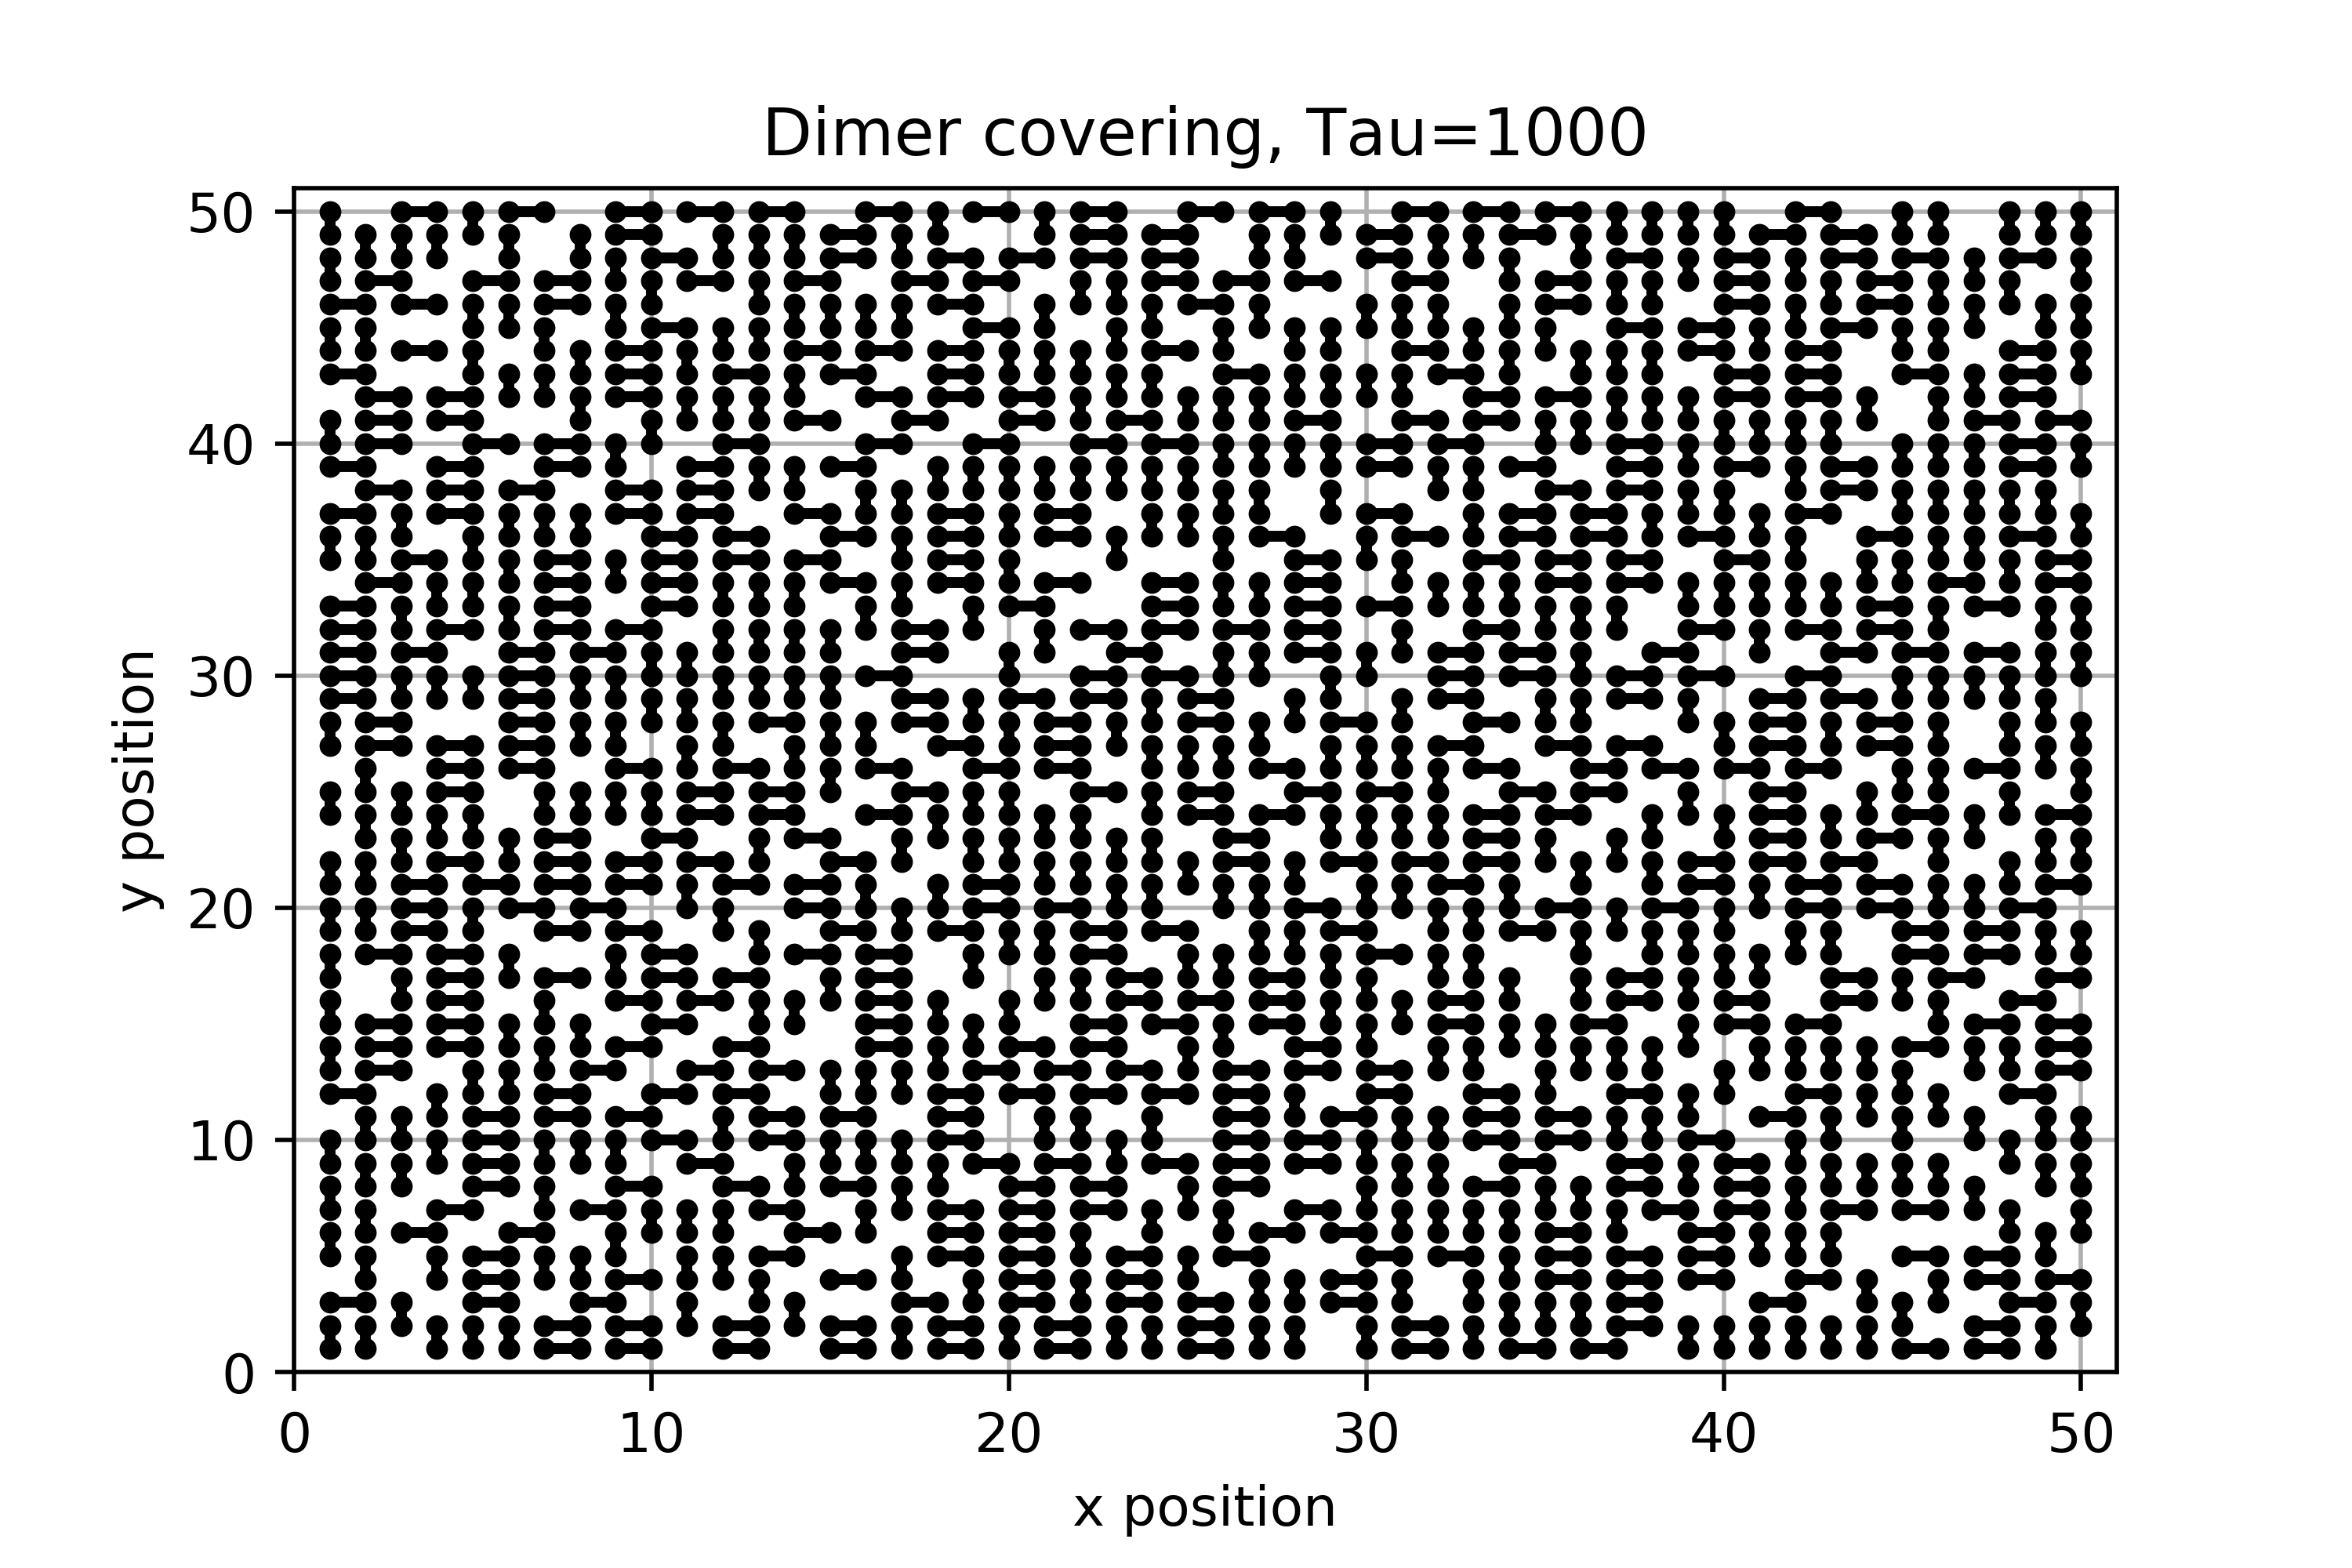
\includegraphics[width=\linewidth]{../images/q4_dimers_t=1e3.png}
	\end{minipage}
	\begin{minipage}{0.49\linewidth}
		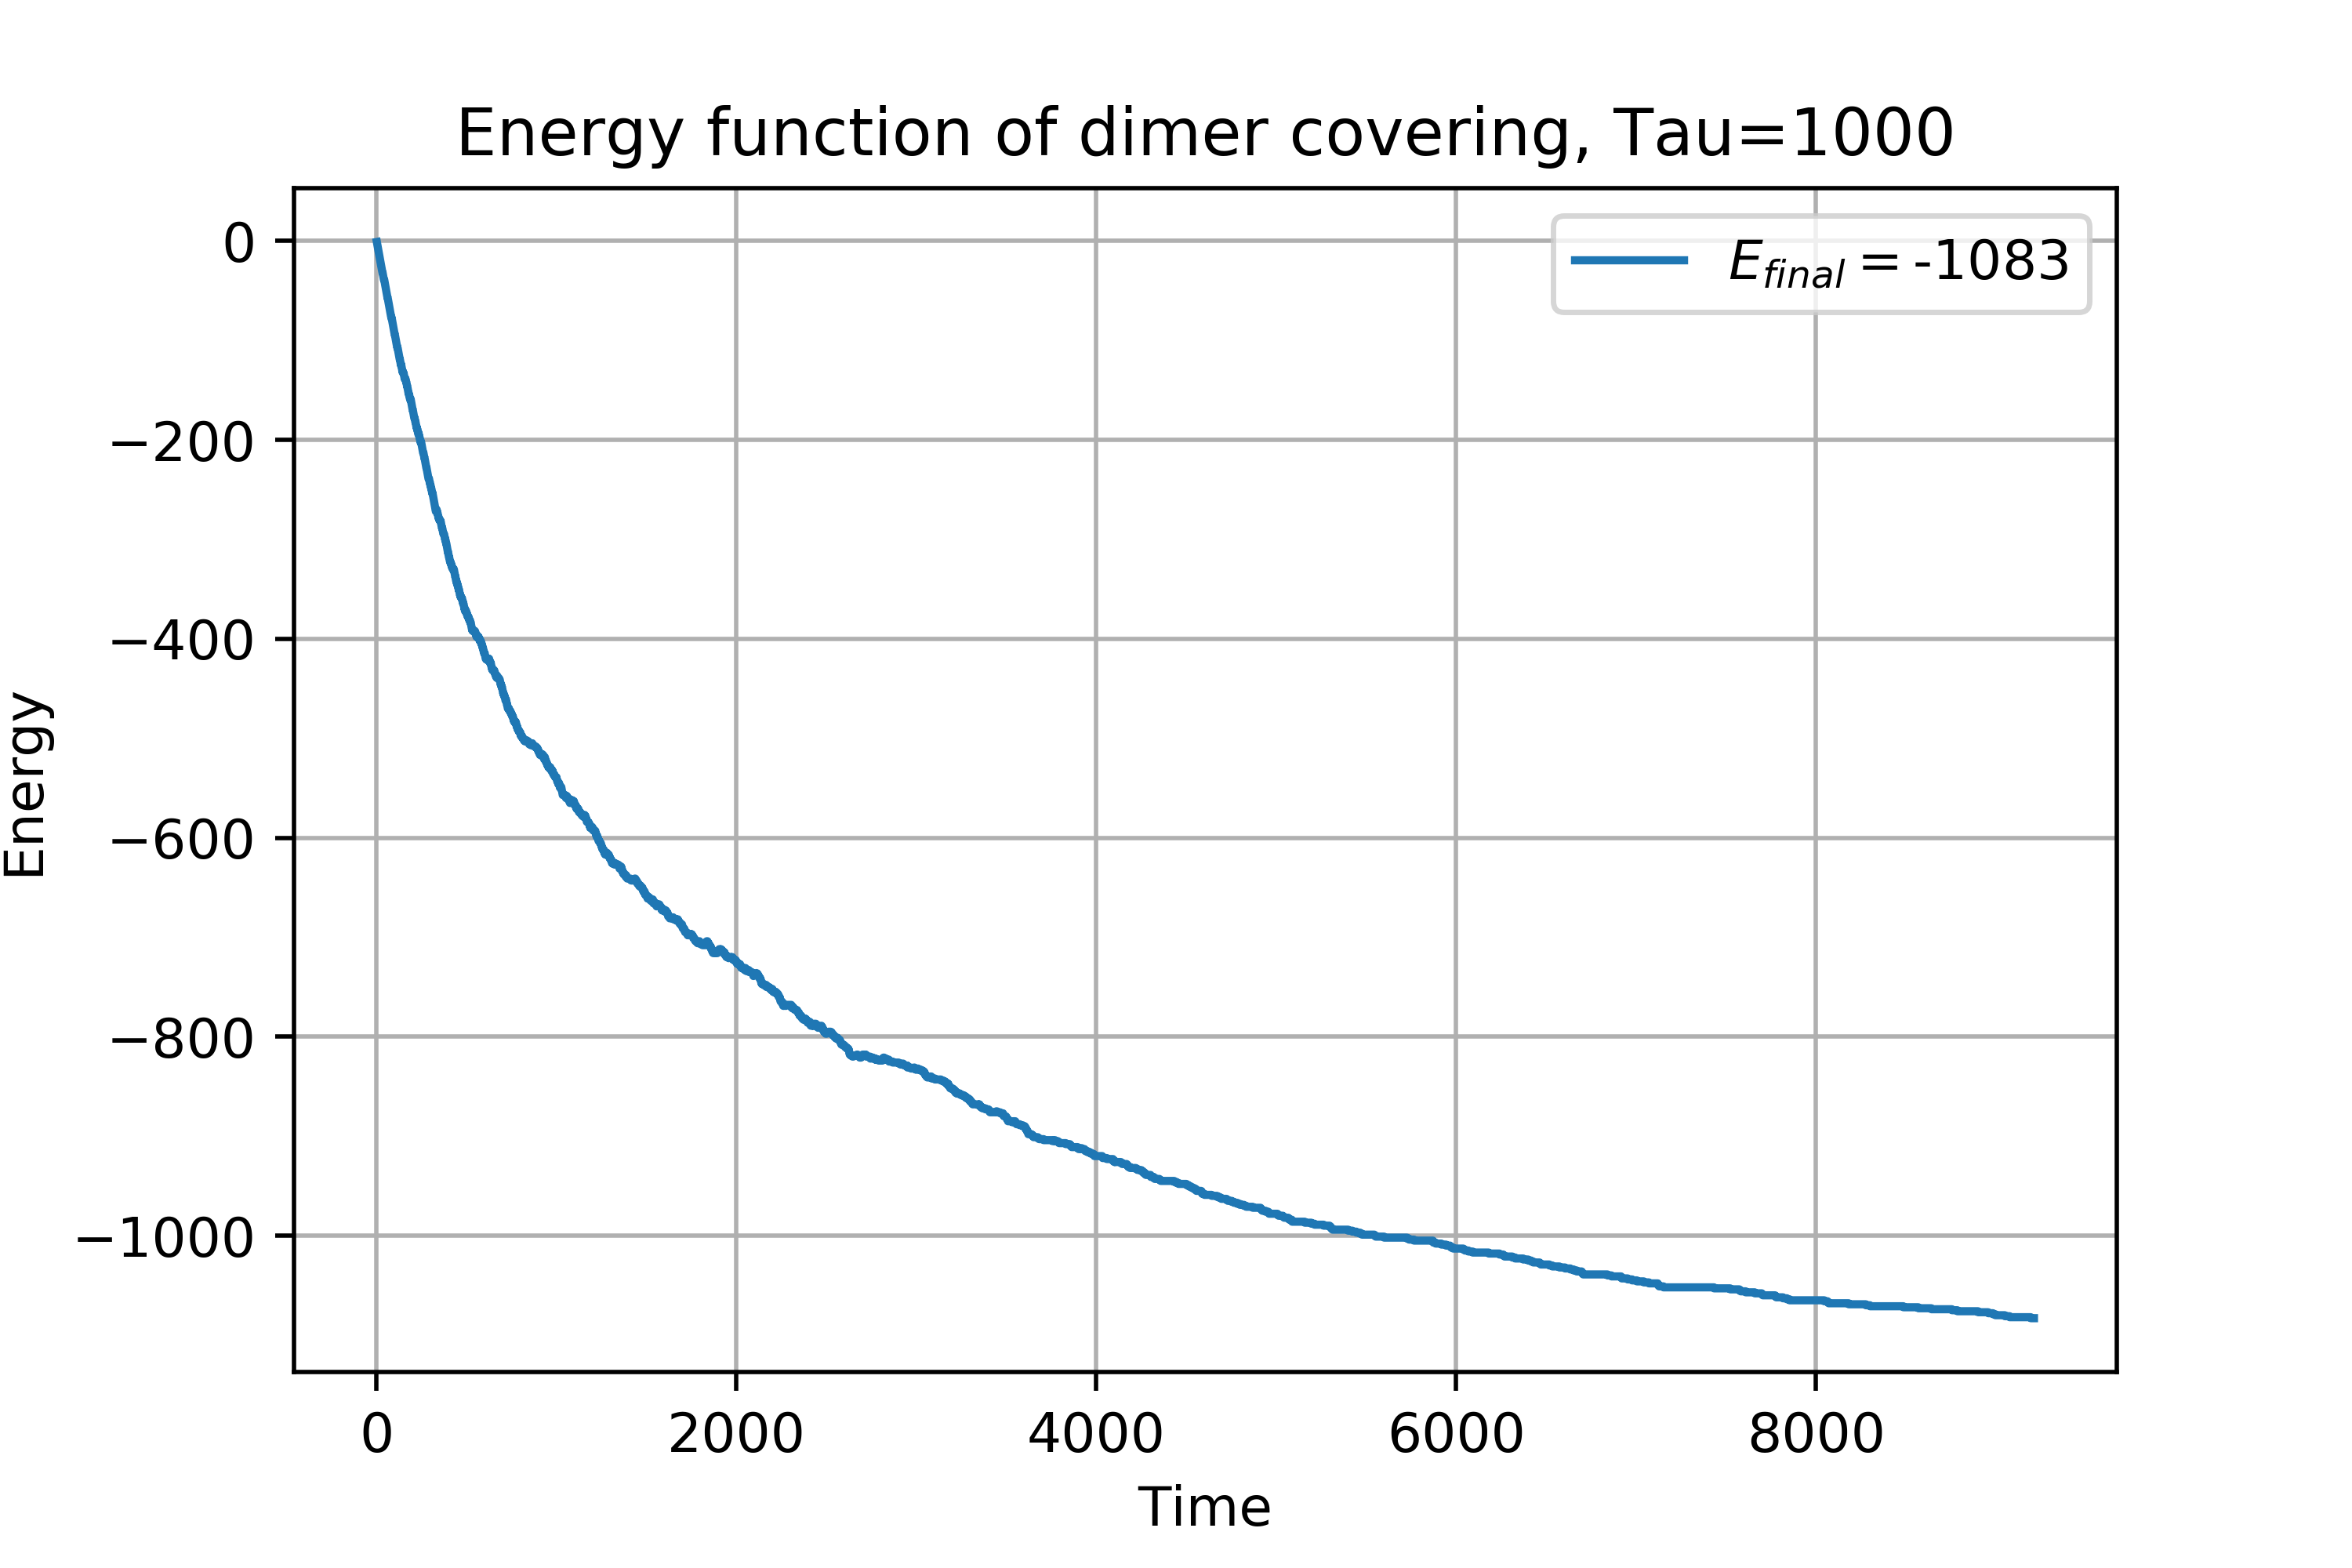
\includegraphics[width=\linewidth]{../images/q4_energy_t=1e3.png}
	\end{minipage}
	\caption{Dimer covering and corresponding energy curve as a result of simulated annealing with a time scale of $\tau = 10^3$}
	\label{fig:q4_dimers_t=1e3}
\end{figure}

\begin{figure}[H]
	\begin{minipage}{0.49\linewidth}
		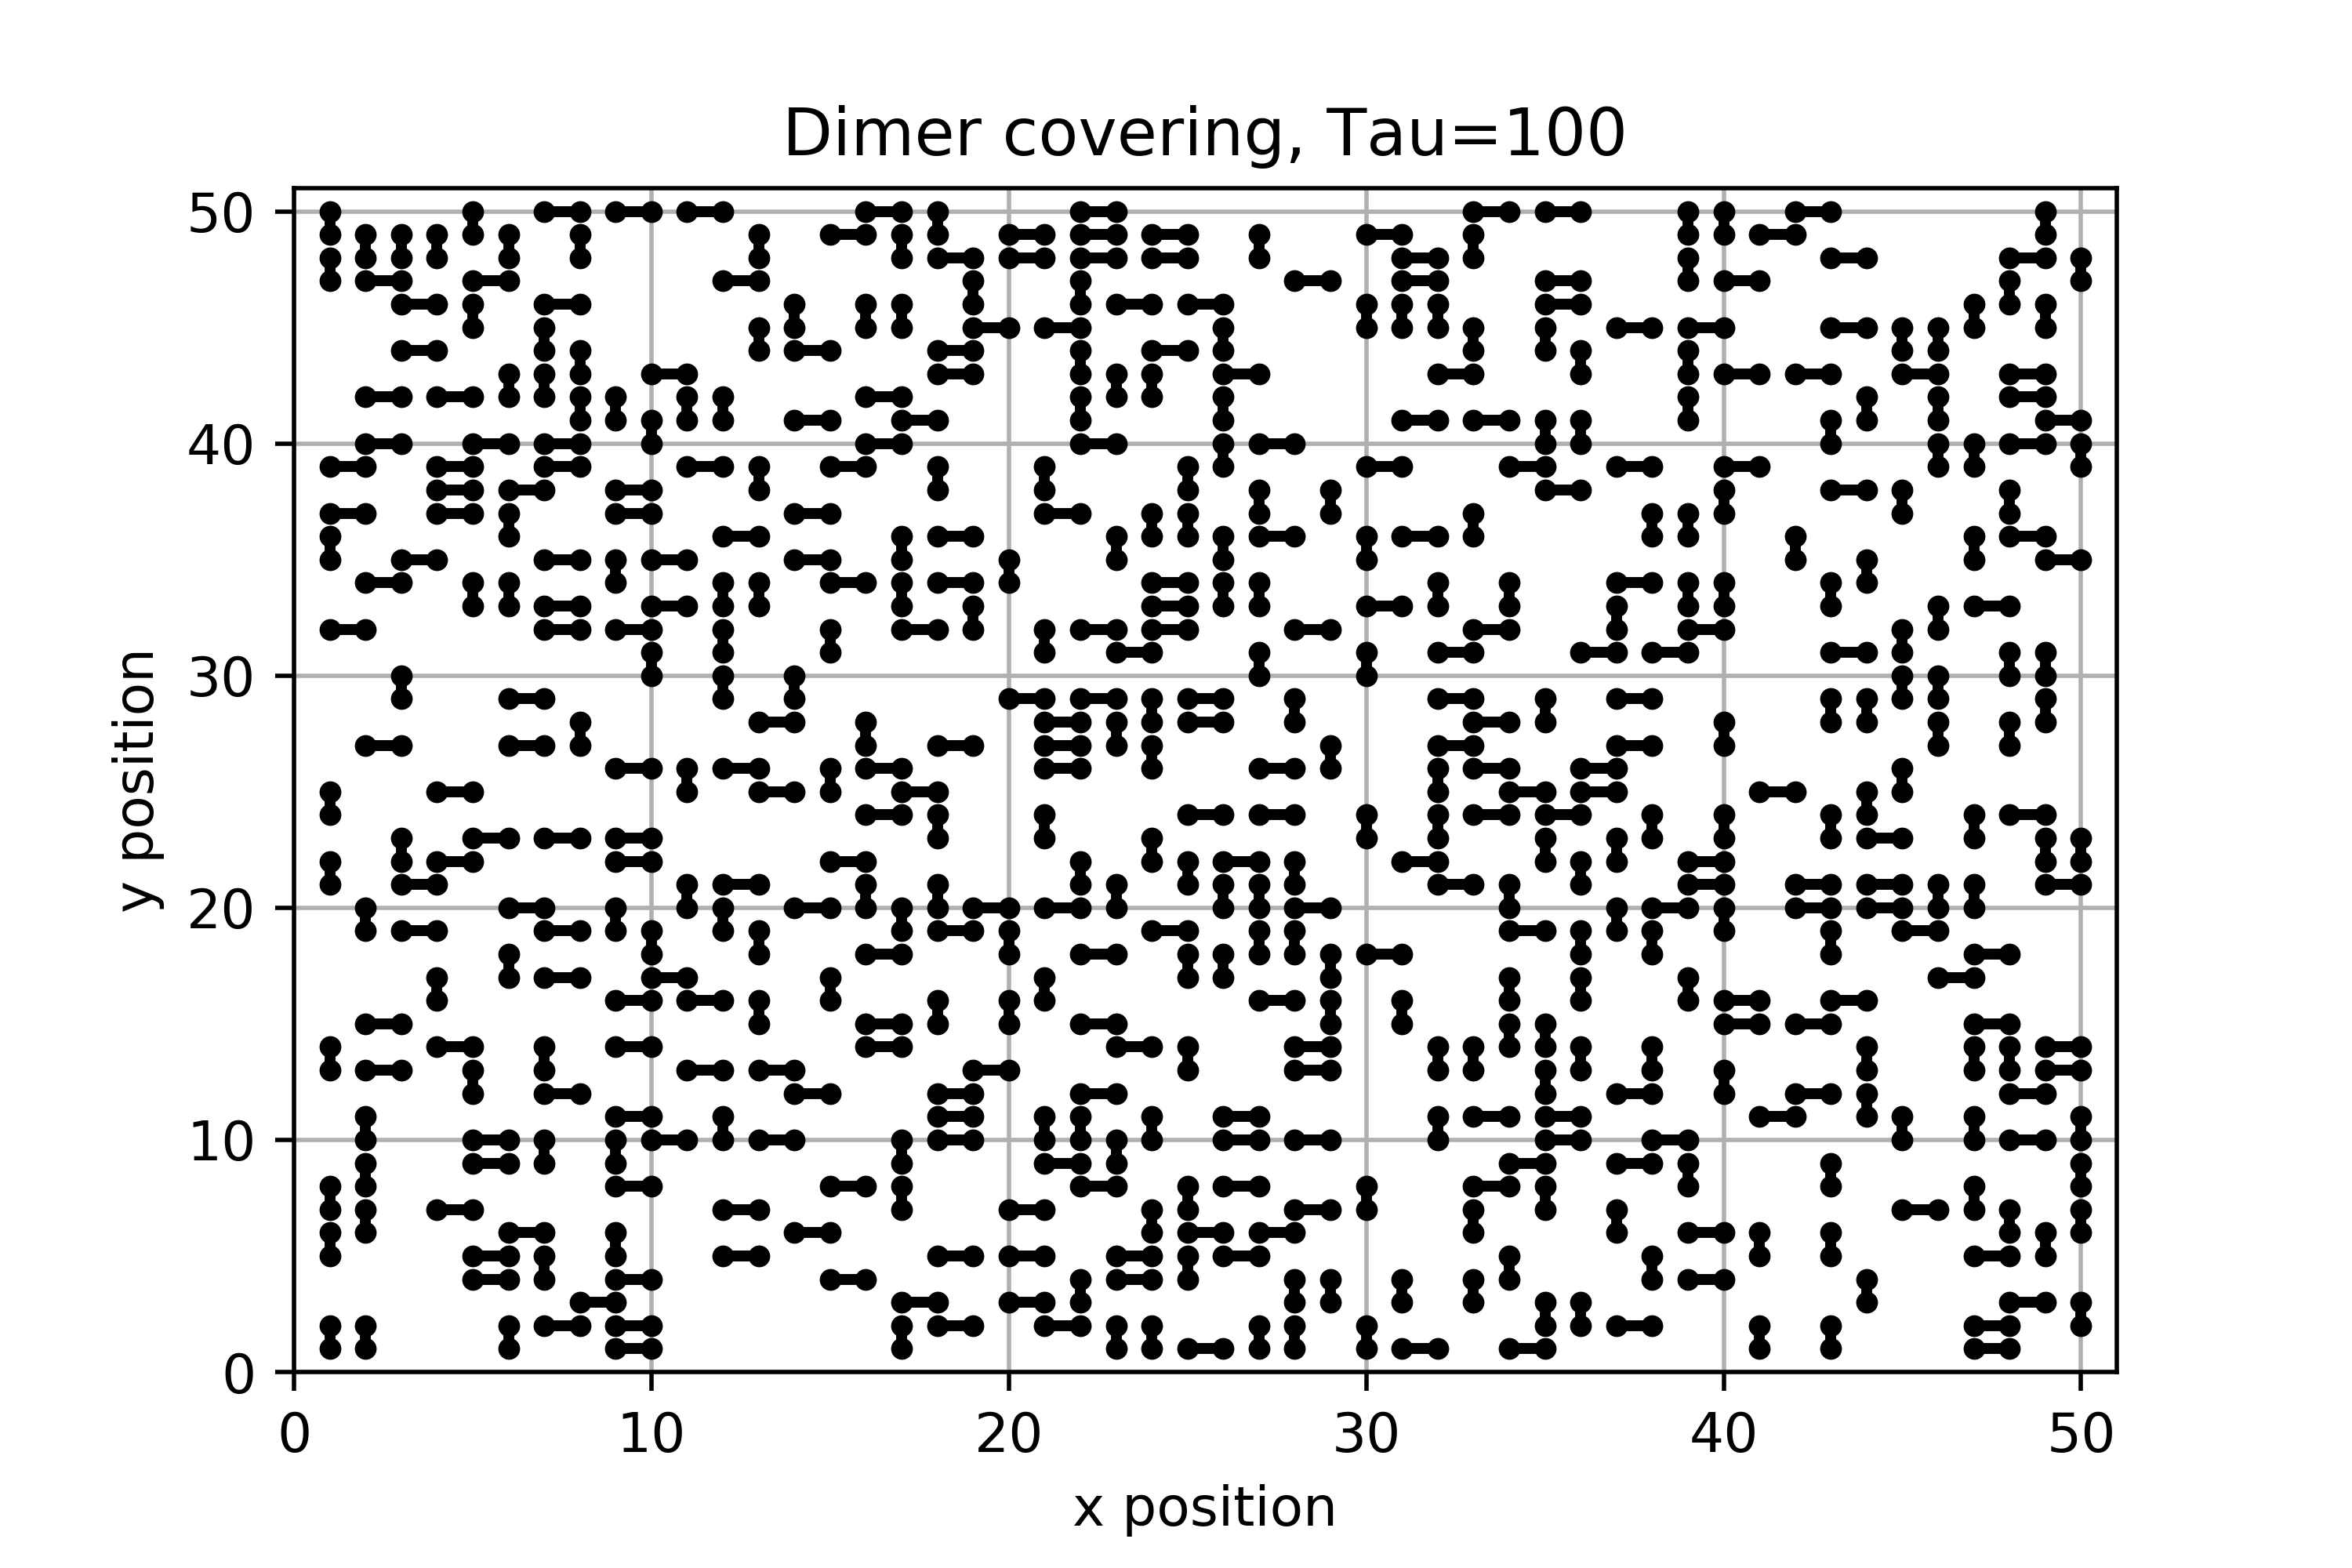
\includegraphics[width=\linewidth]{../images/q4_dimers_t=1e2.png}
	\end{minipage}
	\begin{minipage}{0.49\linewidth}
		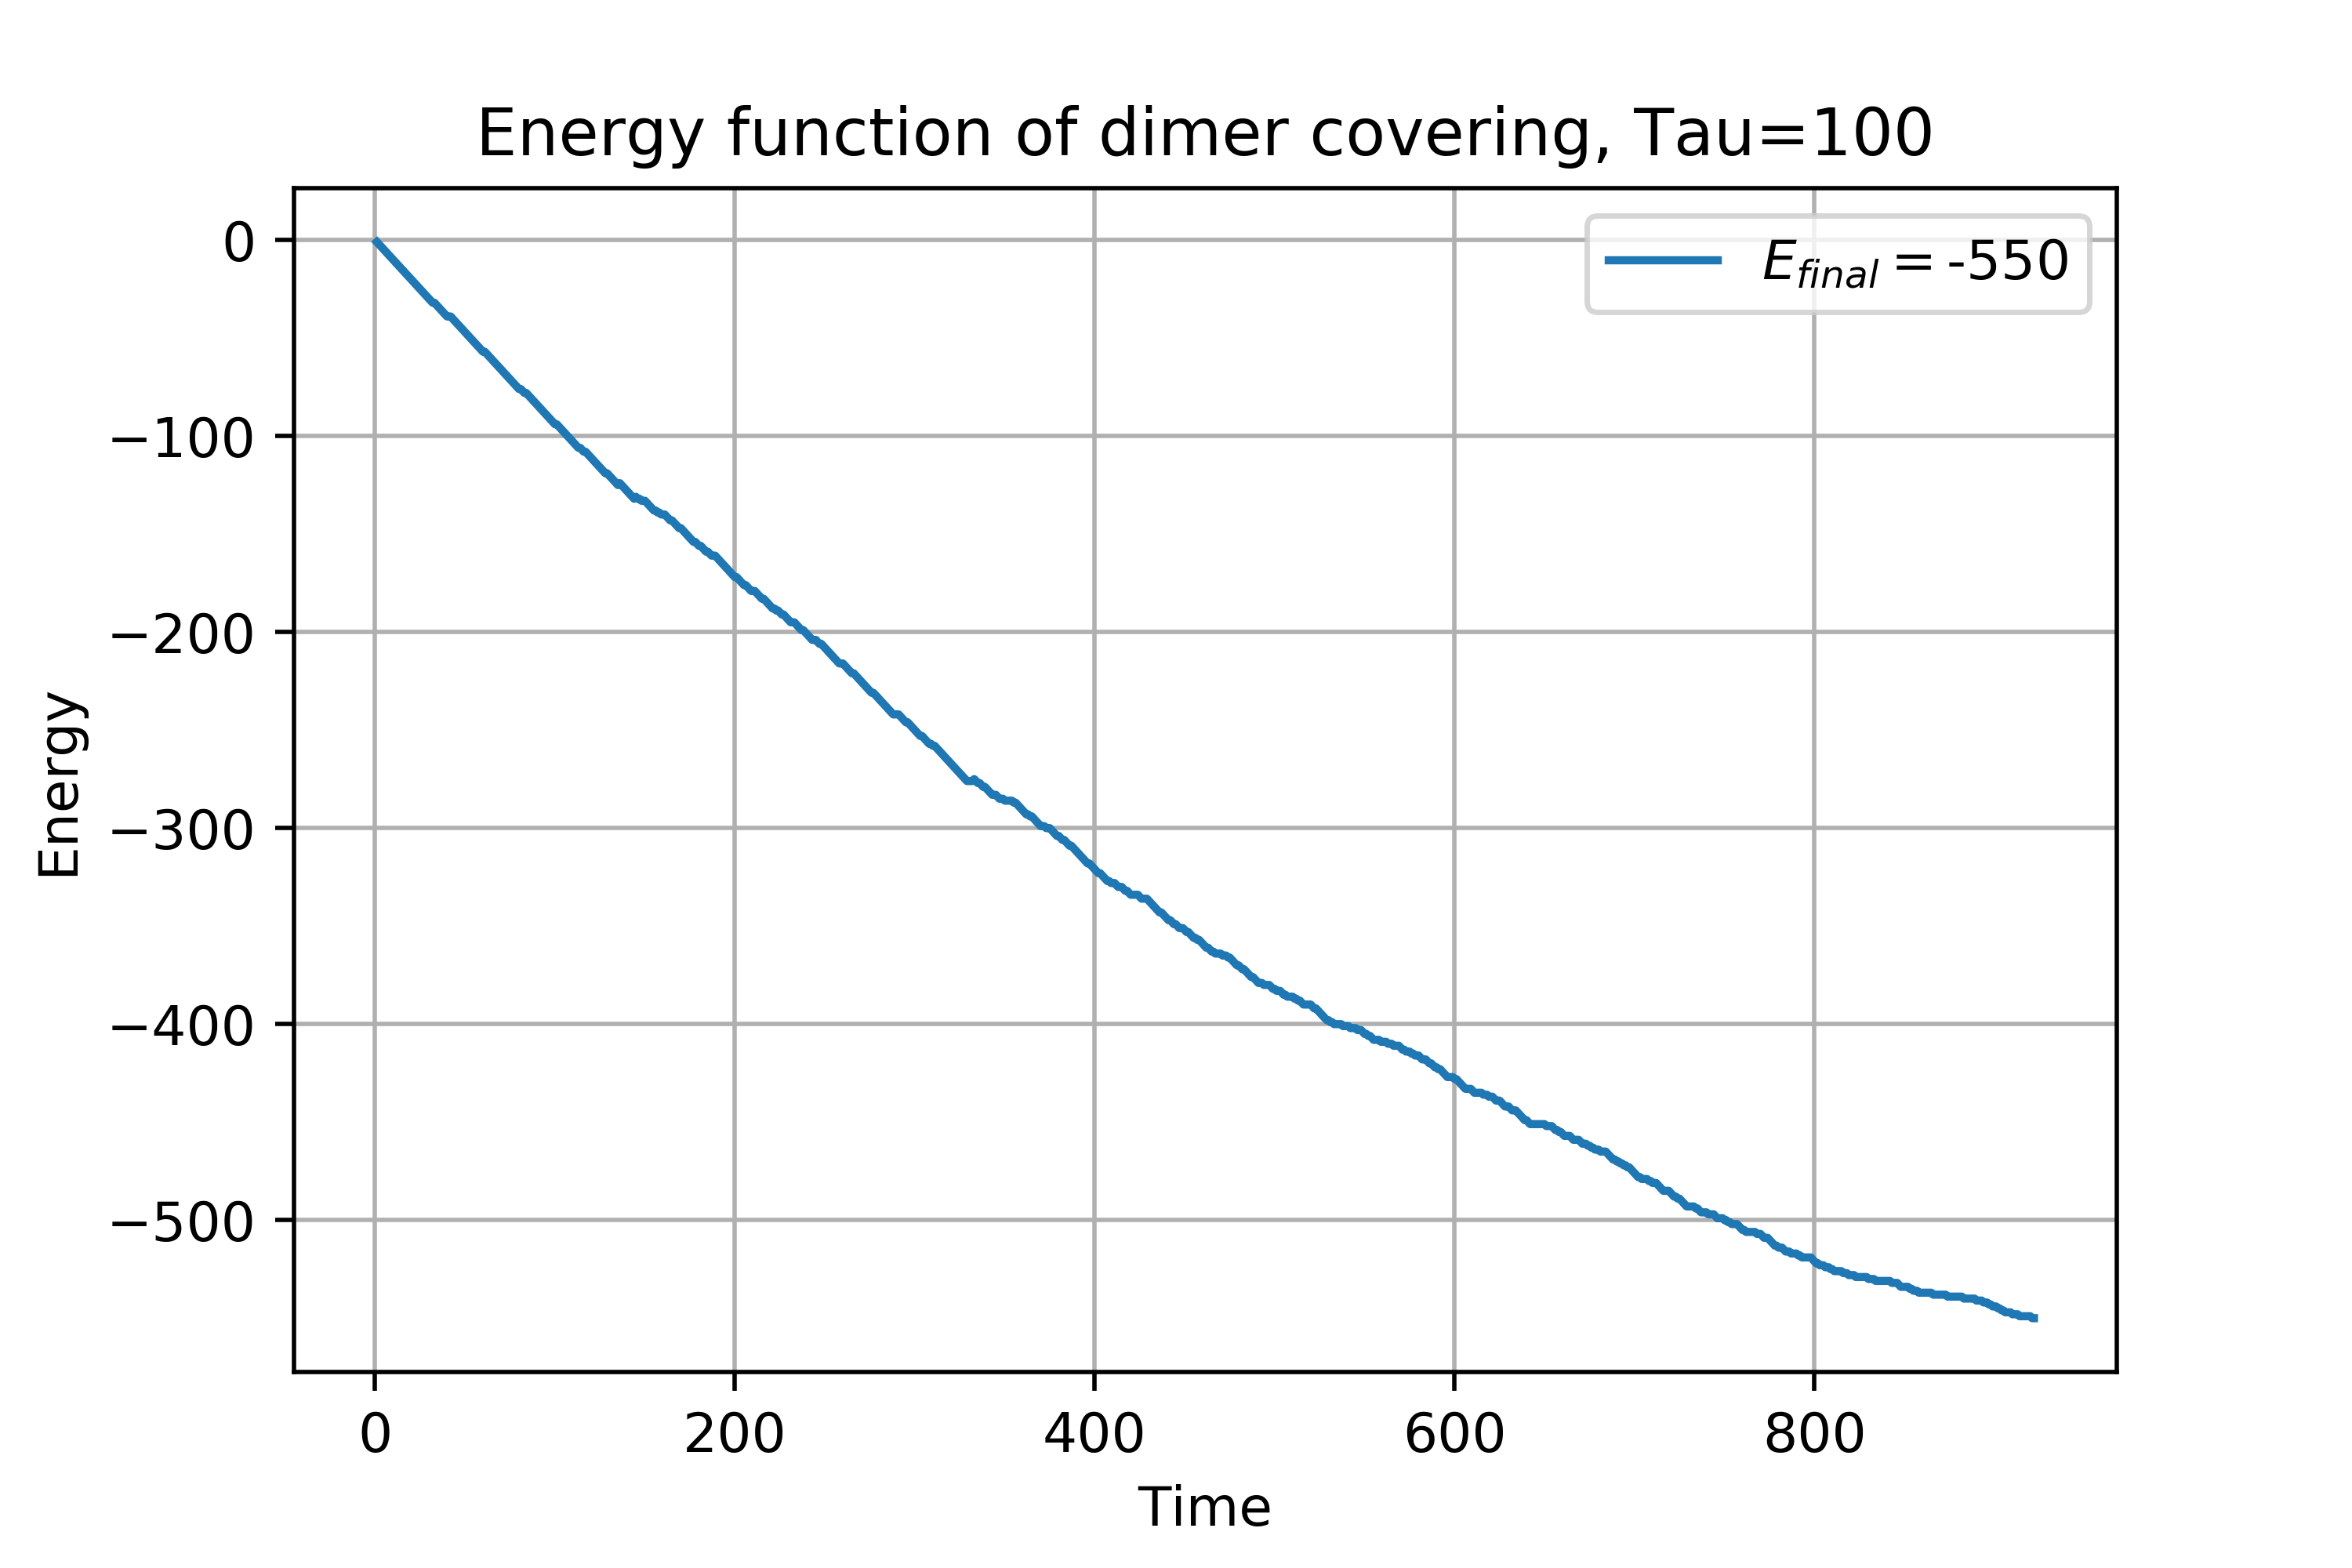
\includegraphics[width=\linewidth]{../images/q4_energy_t=1e2.png}
	\end{minipage}
	\caption{Dimer covering and corresponding energy curve as a result of simulated annealing with a time scale of $\tau = 10^2$}
	\label{fig:q4_dimers_t=1e2}
\end{figure}

\begin{figure}[H]
	\begin{minipage}{0.49\linewidth}
		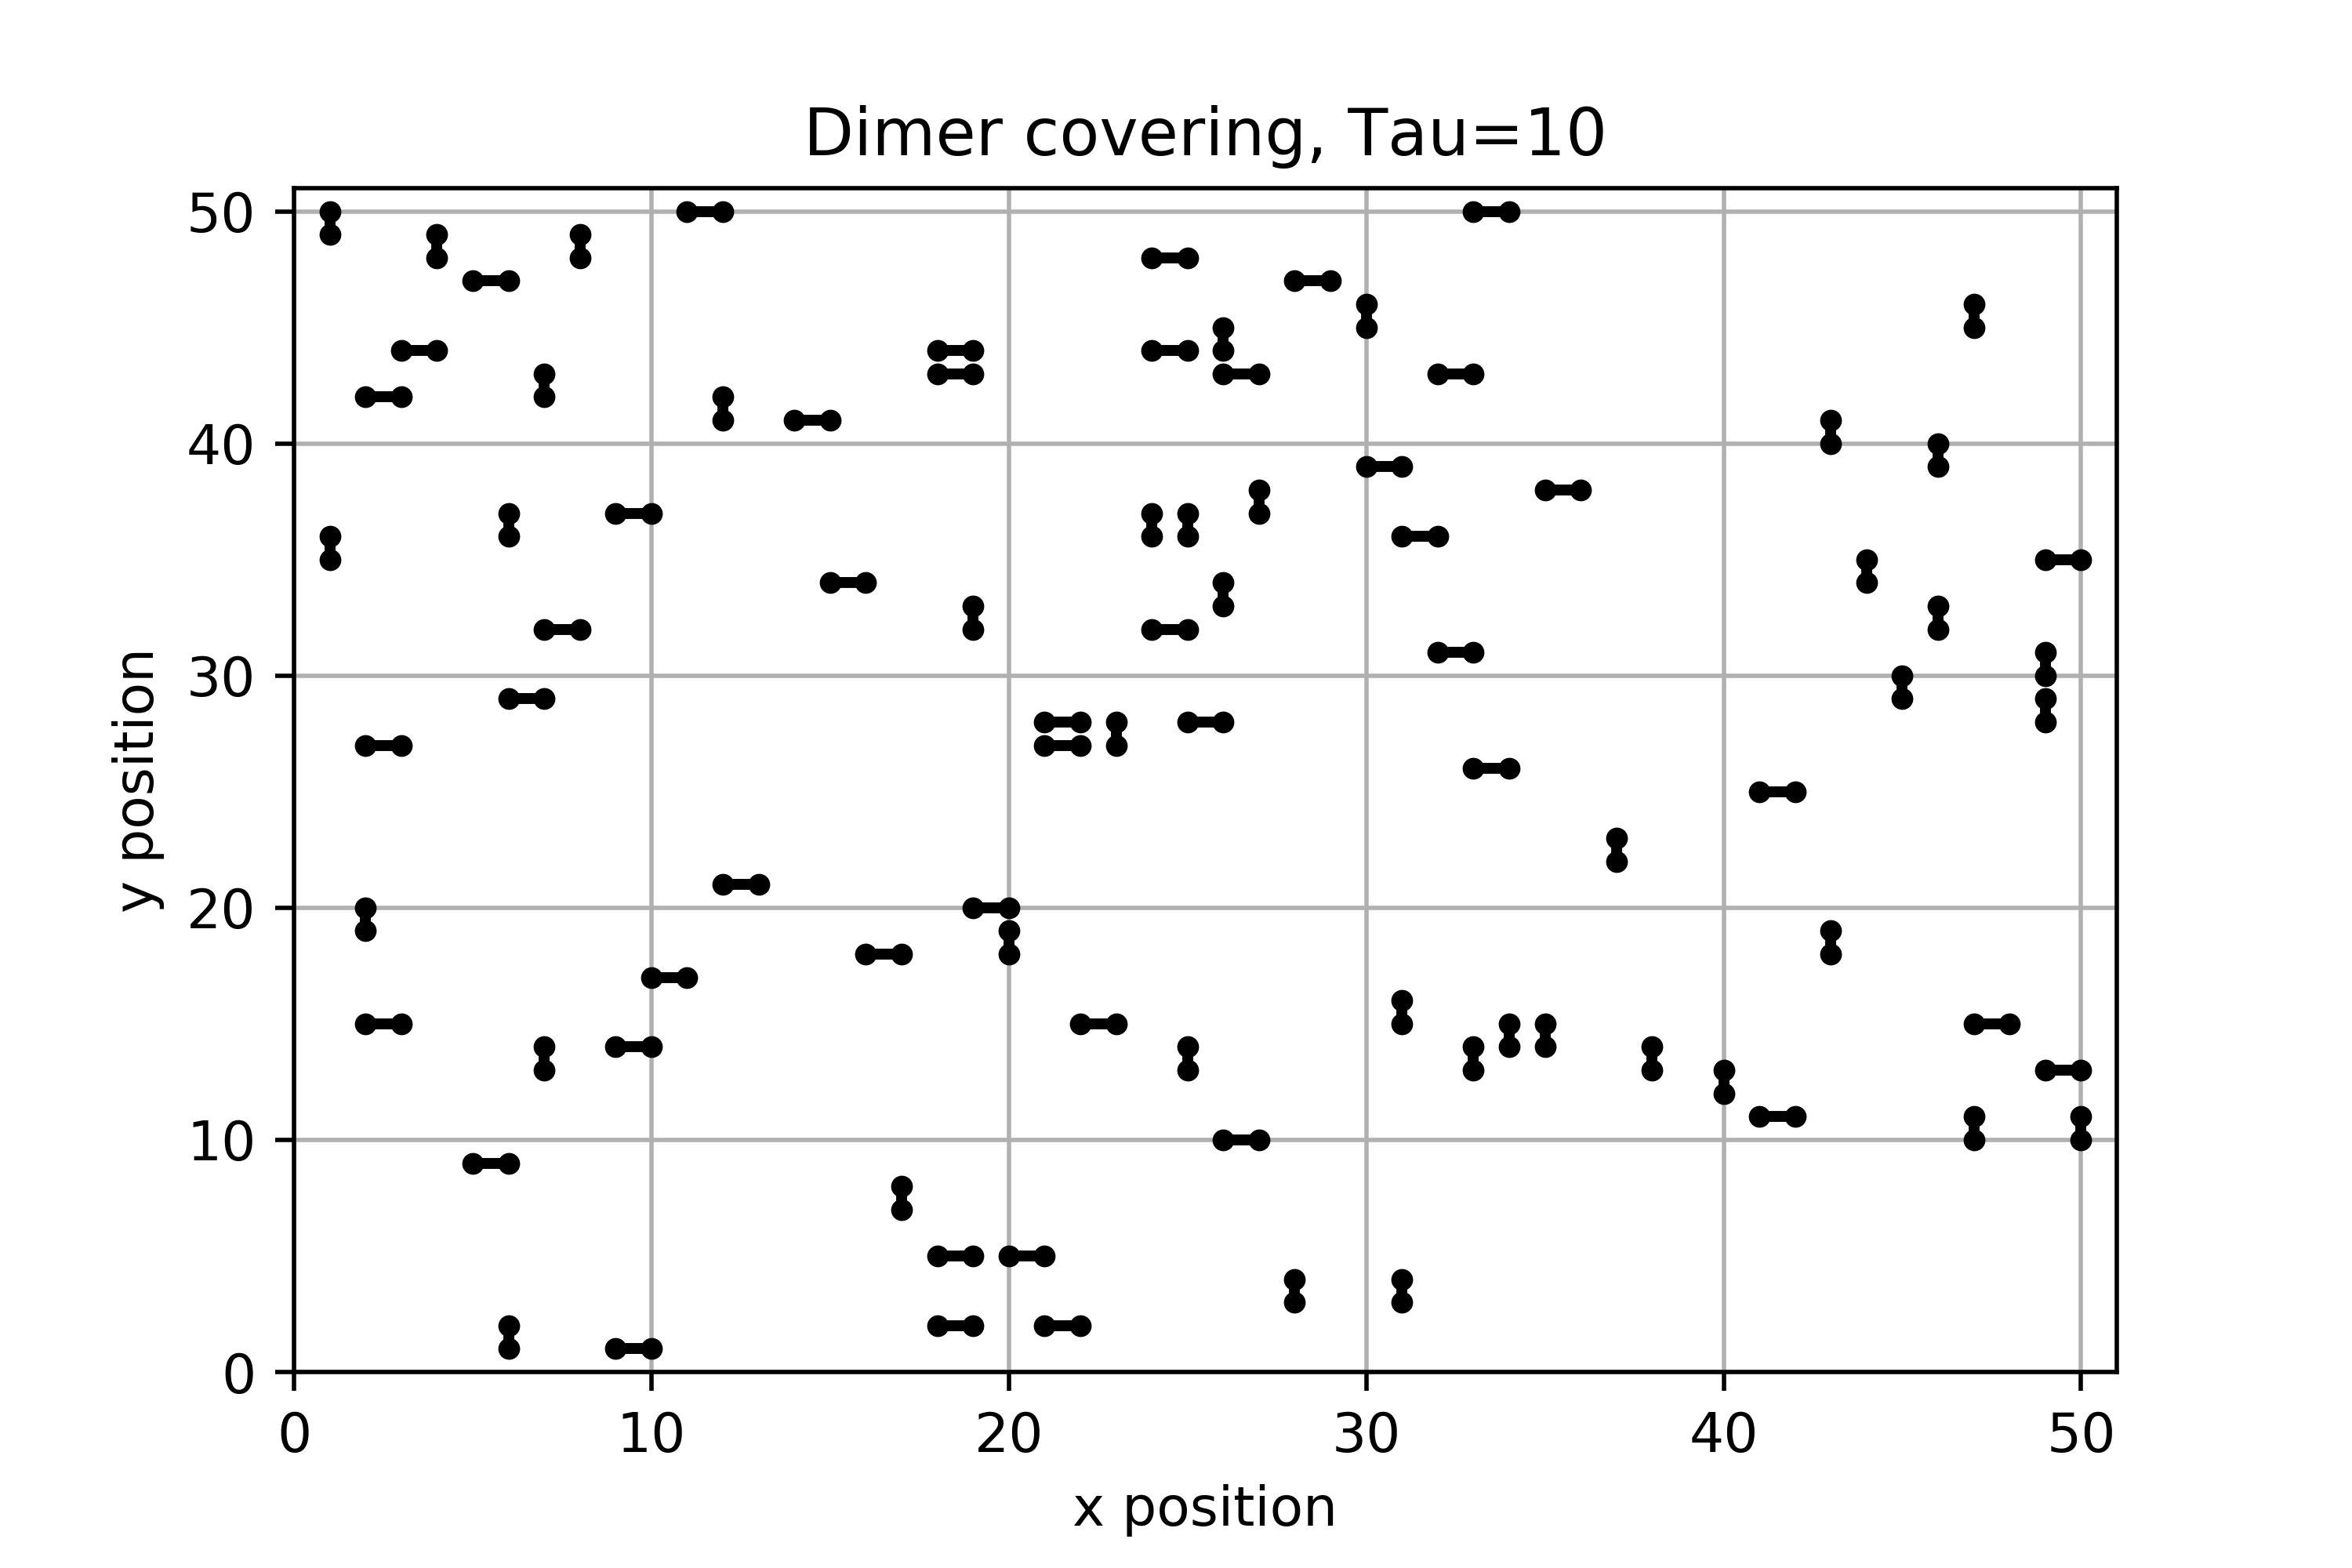
\includegraphics[width=\linewidth]{../images/q4_dimers_t=1e1.png}
	\end{minipage}
	\begin{minipage}{0.49\linewidth}
		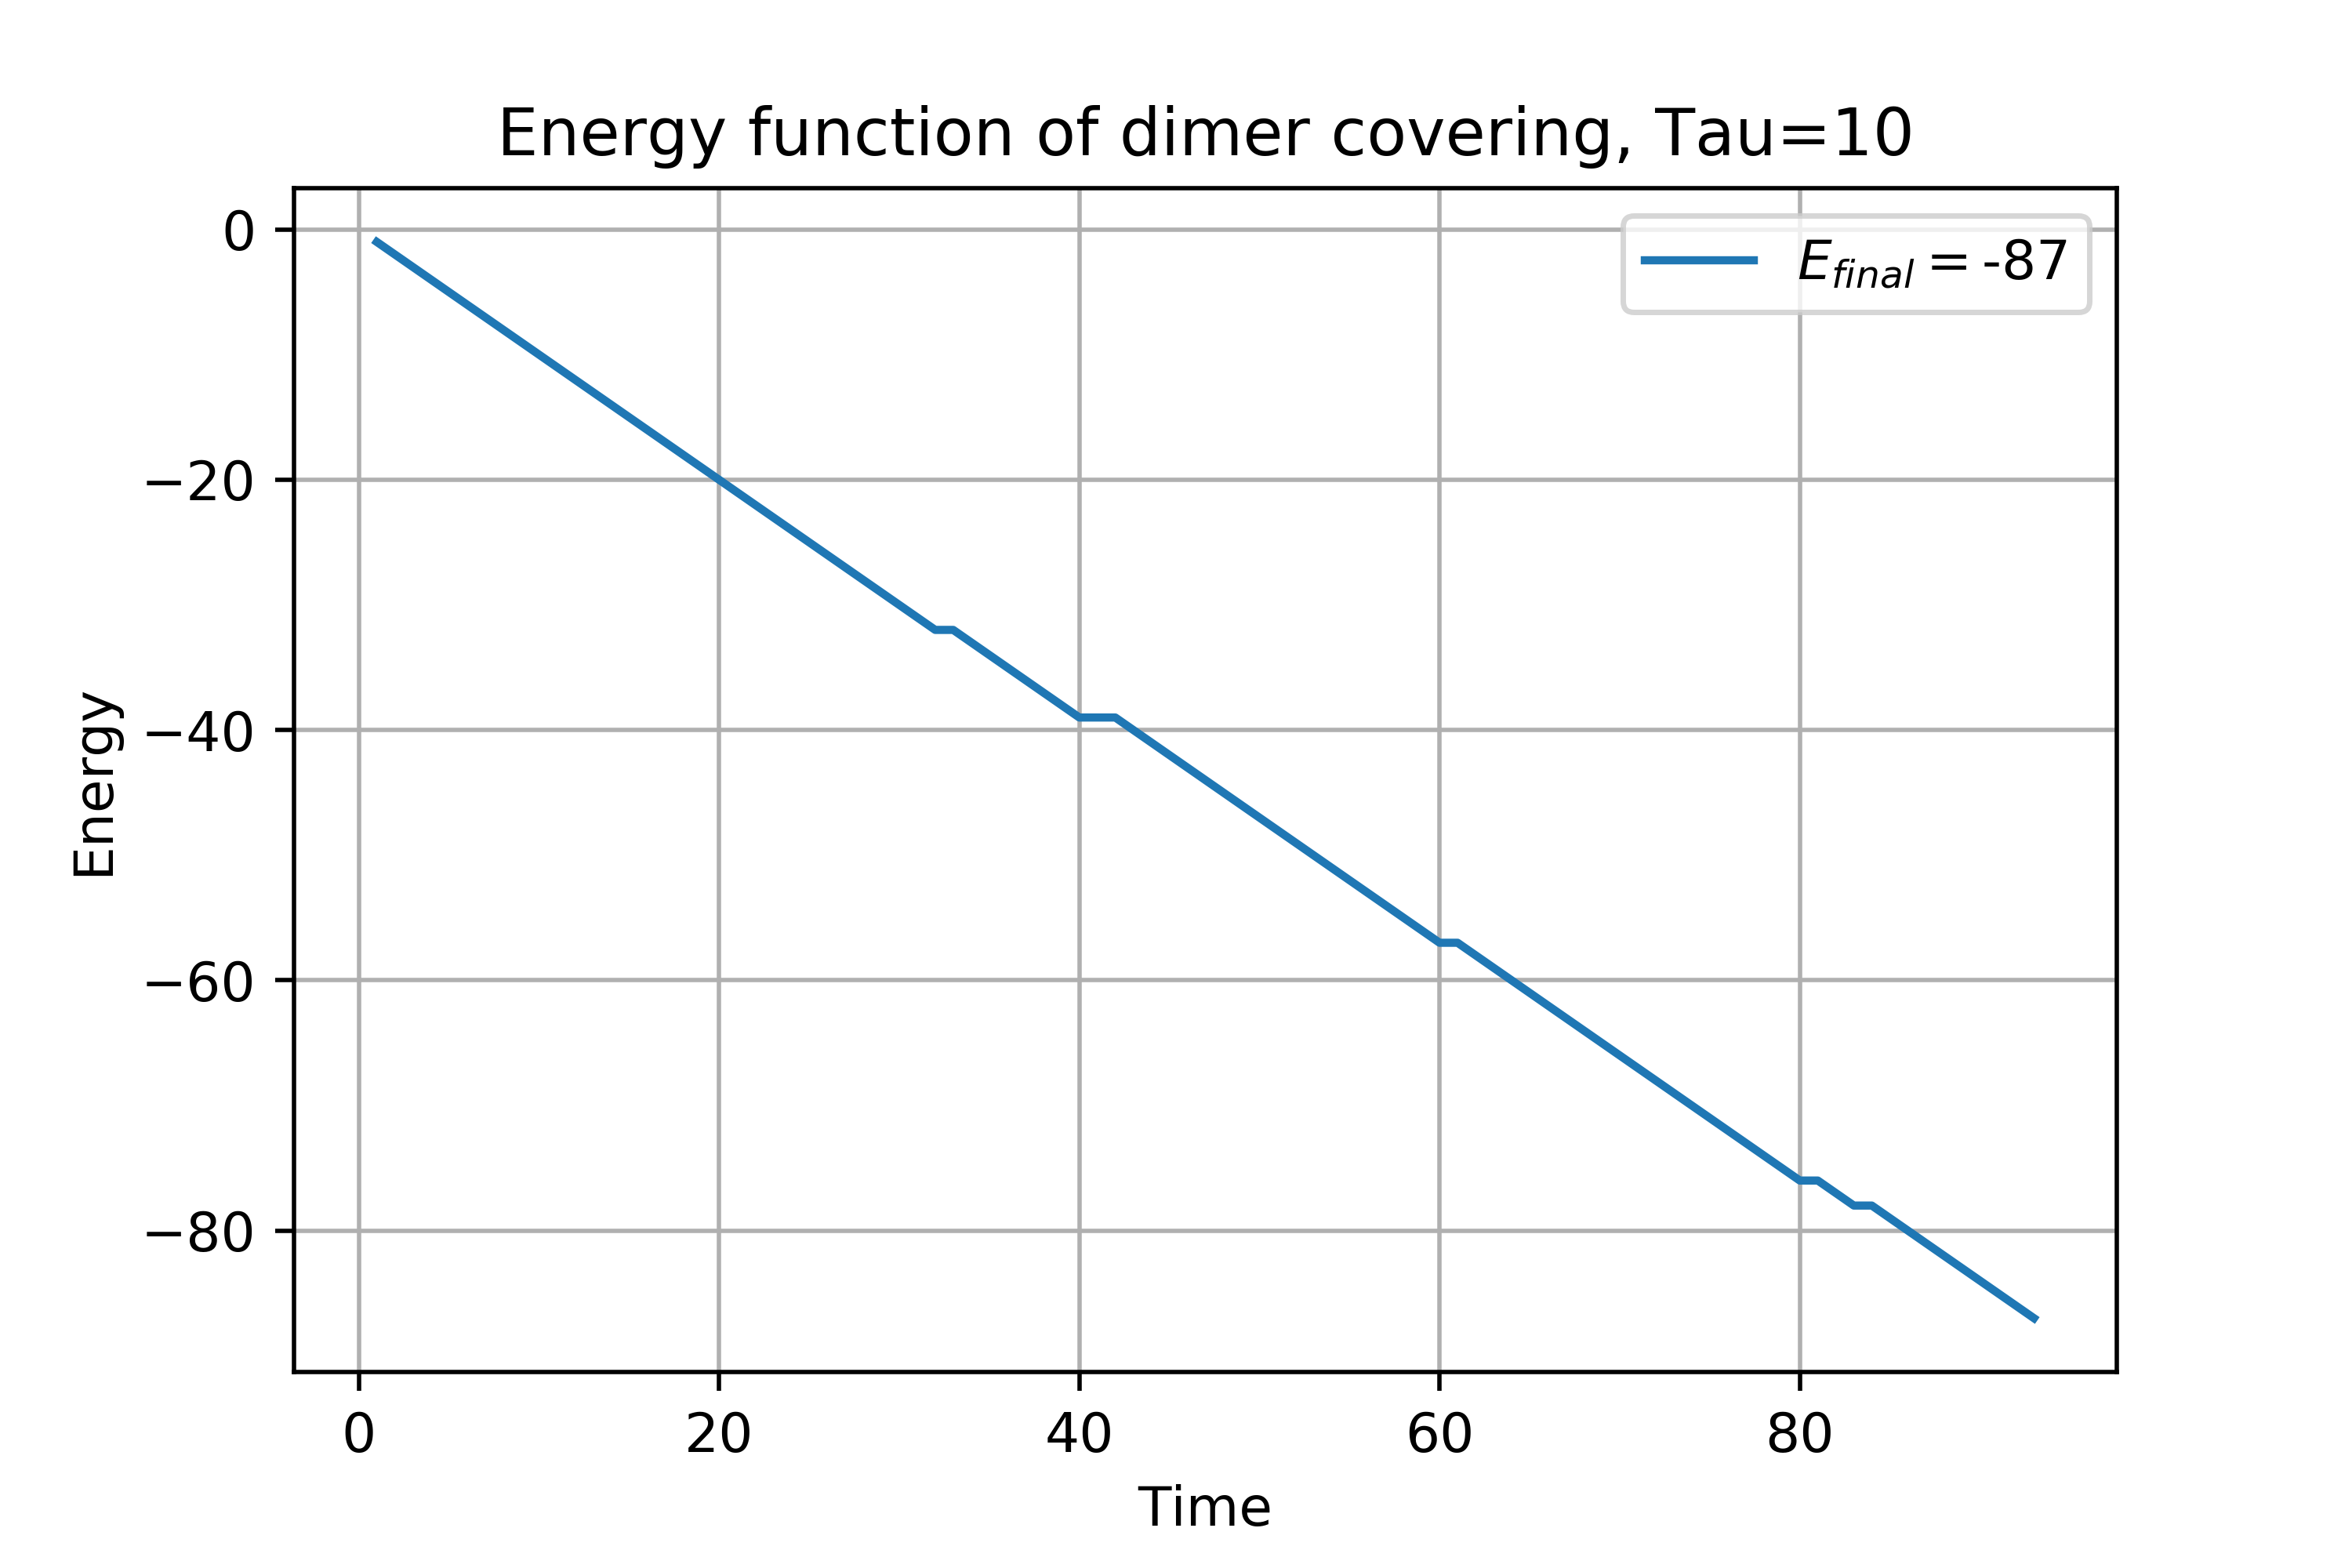
\includegraphics[width=\linewidth]{../images/q4_energy_t=1e1.png}
	\end{minipage}
	\caption{Dimer covering and corresponding energy curve as a result of simulated annealing with a time scale of $\tau = 10$}
	\label{fig:q4_dimers_t=1e1}
\end{figure}

\end{document}